\documentclass[12pt,a4paper]{article}

% ===== Ngôn ngữ & Font Unicode =====
\usepackage{fontspec}              % Dùng Unicode font (bắt buộc với XeLaTeX)
\setmainfont{Times New Roman}      % Có thể đổi: Arial, Roboto, DejaVu Serif,...
\usepackage{xcolor}                % Cho màu chữ
\usepackage{polyglossia}           % Hỗ trợ ngôn ngữ
\setdefaultlanguage{vietnamese}    % Tiếng Việt chuẩn Unicode

% ===== Bố cục trang =====
\usepackage{geometry}
\usepackage{float}
\geometry{
  a4paper,
  left=20mm, right=20mm,
  top=20mm,  bottom=25mm,
  includehead, includefoot,
  headheight=40pt,
  headsep=6mm,
  footskip=12mm
}

% ===== Gói thường dùng =====
\usepackage{graphicx}
\usepackage{longtable,booktabs,array,multirow}
\usepackage{amsmath,amssymb}
\usepackage{fancyhdr}
\usepackage{hyperref}
\usepackage{lastpage}
\usepackage{enumitem}
\usepackage{pdfpages}
\raggedbottom
\usepackage{makecell}
\usepackage{ragged2e}
\usepackage{array}

% ===== Định dạng tiêu đề =====
\usepackage{titlesec}
\titleformat{\section}{\normalfont\Large\bfseries}{\thesection}{0.7em}{}
\titleformat{\subsection}{\normalfont\large\bfseries}{\thesubsection}{0.6em}{}

% ===== Header / Footer =====
\setlength{\headheight}{40pt}
\pagestyle{fancy}
\fancyhead{}
\fancyhead[L]{
 \begin{tabular}{rl}
   
\includegraphics[width=8mm]{hcmut.jpg} &
   \begin{tabular}{l}
     \textbf{Trường Đại học Bách khoa - ĐHQG TP.HCM}\\
     \textbf{Khoa Khoa học và Kỹ thuật Máy tính}
   \end{tabular}
 \end{tabular}
}
\fancyfoot{}
\fancyfoot[R]{\scriptsize Trang \thepage/\pageref{LastPage}}
\renewcommand{\headrulewidth}{0.3pt}
\renewcommand{\footrulewidth}{0.3pt}

\begin{document}

% ===== Trang bìa =====
\begin{titlepage}
\begin{center}
{\large ĐẠI HỌC QUỐC GIA THÀNH PHỐ HỒ CHÍ MINH}\\
{\large TRƯỜNG ĐẠI HỌC BÁCH KHOA}\\
{\large KHOA KHOA HỌC VÀ KỸ THUẬT MÁY TÍNH}\\[1cm]


\includegraphics[width=4cm]{hcmut.jpg}

\vspace{1cm}
{\LARGE \textbf{MẠNG MÁY TÍNH}}\\[0.6cm]
{\Large \textbf{BÀI TẬP LỚN}}\\[0.5cm]
{\Large \textbf{LỚP L07 - NHÓM XX}}\\[0.2cm]
{\large Học kỳ 251}\\[1cm]
\textbf{GVHD: BÙI XUÂN GIANG}

\vfill
{\footnotesize TP. Hồ Chí Minh, Tháng 11/2025}
\end{center}
\end{titlepage}

% ===== Mục lục =====
\tableofcontents
\newpage

% ===== Bảng phân công (4 người) =====
\section*{Bảng phân công nhiệm vụ}
\addcontentsline{toc}{section}{Bảng phân công nhiệm vụ}
\renewcommand{\arraystretch}{1.5}
\setlength{\tabcolsep}{6pt}
\small
\begin{longtable}{
  |>{\centering\arraybackslash}m{0.8cm}| 
  >{\centering\arraybackslash}m{3.4cm}| 
  >{\centering\arraybackslash}m{1.8cm}| 
  >{\arraybackslash}m{8.2cm}| 
  >{\centering\arraybackslash}m{1.4cm}|
}
\hline
\textbf{STT} & \textbf{Họ và Tên} & \textbf{MSSV} & \centering\textbf{Nhiệm vụ chính} & \textbf{Hoàn thành} \\
\hline
\endfirsthead

\hline
\textbf{STT} & \textbf{Họ và Tên} & \textbf{MSSV} & \centering\textbf{Nhiệm vụ chính} & \textbf{Hoàn thành} \\
\hline
\endhead

\makecell{1} & \makecell{Nguyễn Minh Hạnh} & \makecell{2310895} &
\makecell[l]{
-- Thực hiện phần Peer-to-Peer (P2P)\\
-- Viết báo cáo
} &
\makecell{100\%} \\ \hline

\makecell{2} & \makecell{Trần Đình Hoàng} & \makecell{2311075} &
\makecell[l]{
-- Tổng hợp code\\
-- Chạy test\\
-- Viết báo cáo
} &
\makecell{100\%} \\ \hline

\makecell{3} & \makecell{Trương Hoàng Thông} & \makecell{2313336} &
\makecell[l]{
-- Thực hiện phần Client--Server
} &
\makecell{100\%} \\ \hline

\makecell{4} & \makecell{Nguyễn Lê Anh Xuân} & \makecell{2420013} &
\makecell[l]{
-- Thực hiện phần Cookies và Session
} &
\makecell{100\%} \\ \hline

\end{longtable}
\normalsize
\newpage

% ======================================================================
\section{Lời mở đầu}
\subsection{Tổng quan bài tập lớn}

Bài tập lớn 1 yêu cầu sinh viên hiện thực một hệ thống mô phỏng hoạt động kết hợp giữa HTTP Server (Client–Server paradigm) và mô hình Peer-to-Peer (P2P paradigm). Hệ thống cho phép các peer đăng ký, kết nối và gửi tin nhắn trực tiếp thông qua backend trung gian đóng vai trò như một tracker.

\subsection{Mục tiêu và kết quả đạt được}

Mục tiêu của bài tập này là giúp sinh viên vận dụng các thành phần quan trọng trong một hệ thống mạng máy tính, chẳng hạn như mô hình Client–Server, mô hình Peer-to-Peer (P2P) và lập trình mạng (Network Programming).

Cụ thể, sinh viên sẽ thực hành với ba mô-đun chính là giao tiếp HTTP theo mô hình Client–Server, ứng dụng chat dựa trên mô hình Peer-to-Peer, kết nối mạng TCP/IP, bao gồm
\begin{itemize}
    \item Các tiến trình client và server.
    \item Nhiều tiến trình peer có khả năng kết nối với nhau.
    \item Lập trình mạng bằng socket TCP.
\end{itemize}
Ngoài ra, sinh viên sẽ thực hành thiết kế và hiện thực một giao thức P2P đơn giản hoạt động trên nền TCP/IP.

Sau khi hoàn thành bài tập này, sinh viên có thể hiểu một phần nguyên lý hoạt động của hệ thống mạng máy tính, sẽ nắm được vai trò và cách thiết kế của các loại tiến trình trong quá trình giao tiếp mạng, bao gồm server process, client process, và tracker peer process trong mô hình truyền thông mạng.
% ======================================================================
\section{Cơ sở lý thuyết – Giải pháp đề xuất}
\subsection{Mô hình Client-Server}

Client server là mô hình mạng máy tính gồm có 2 thành phần chính đó là máy khách (client) và máy chủ (server). Server chính là nơi giúp lưu trữ tài nguyên cũng như cài đặt các chương trình dịch vụ theo đúng như yêu cầu của client. Ngược lại, Client bao gồm máy tính cũng như các loại thiết bị điện tử nói chung sẽ tiến hành gửi yêu cầu đến server.\\
Mô hình mạng Client-Server sẽ cho phép mạng tập trung các ứng dụng có cùng chức năng tại một hoặc nhiều dịch vụ file chuyên dụng. Chúng sẽ trở thành trung tâm của hệ thống. Hệ điều hành của mô hình Client-server sẽ cho phép người dùng chia sẻ đồng thời cùng một loại tài nguyên mà không giới hạn vị trí địa lý. 
\subsection{Mô hình Peer-to-Peer (P2P)}

 Mạng Peer-to-Peer (P2P) là một mô hình mạng trong đó các máy tính (gọi là peer) kết nối và chia sẻ tài nguyên trực tiếp với nhau mà không cần thông qua một máy chủ trung gian. Trong mạng này, mỗi peer có thể vừa là máy khách (client) vừa là máy chủ (server), giúp phân tán tài nguyên và tăng khả năng chia sẻ dữ liệu một cách hiệu quả. Các peer có thể trao đổi dữ liệu, tệp tin, và tài nguyên khác một cách trực tiếp mà không cần phụ thuộc vào hệ thống tập trung, giúp giảm thiểu tắc nghẽn mạng và tăng khả năng mở rộng. Mạng P2P có thể được phân loại dựa trên cách tổ chức và điều phối các peer: Hai loại chính là mạng P2P tập trung (centralized P2P) và mạng P2P phi tập trung (decentralized P2P).\\
Trong mạng P2P tập trung, một máy chủ trung tâm (tracker) được sử dụng để quản lý danh sách các peer và điều phối kết nối giữa các peer trong mạng. Khi một peer muốn tìm kiếm dữ liệu hoặc tài nguyên, nó sẽ liên hệ với tracker để biết các peer khác đang có dữ liệu mong muốn. Tracker đóng vai trò hỗ trợ việc kết nối ban đầu giữa các peer, sau đó các peer sẽ thực hiện việc truyền dữ liệu trực tiếp với nhau. Mô hình này dễ dàng triển khai và quản lý hơn so với mạng phi tập trung nhưng phụ thuộc vào máy chủ trung tâm, dẫn đến khả năng bị gián đoạn nếu máy chủ bị lỗi.
\subsection{Mô hình hybrid}
Mô hình lai kết hợp ưu điểm của cả Client-Server và P2P, thường được áp dụng trong các ứng dụng chat hoặc chia sẻ tập tin quy mô lớn (ví dụ: BitTorrent).
\begin{itemize}
    \item \textbf{Vai trò Client–Server (Tracker):} Được sử dụng trong giai đoạn \textbf{khởi tạo} (\textit{Initialization}) để quản lý trạng thái, xác thực người dùng và hỗ trợ \textbf{khám phá peer} (\textit{Peer Discovery}) thông qua các API như \texttt{/add-list} và \texttt{/get-list}.
    \item \textbf{Vai trò P2P:} Được sử dụng trong giai đoạn \textbf{trao đổi dữ liệu} (\textit{Data Exchange}). Sau khi có địa chỉ của peer đích, các peer sẽ thiết lập \textbf{kết nối TCP trực tiếp} để trao đổi tin nhắn mà không cần qua server trung tâm, giúp giảm tải cho server và tăng tốc độ truyền tin.
\end{itemize}
\subsection{Cơ chế Cookie và Session}
Trong giao thức HTTP, cookie được sử dụng để lưu trữ thông tin trạng thái của người dùng giữa các request. 
Khi người dùng đăng nhập thành công, server sẽ gửi một cookie chứa mã \texttt{session ID} về cho client. 
Client sẽ đính kèm cookie này trong các yêu cầu tiếp theo để chứng minh trạng thái đăng nhập.
Trong bài tập lớn, module \texttt{session\_store.py} đảm nhận việc tạo và xác thực cookie này.
% \subsection{Proxy}
% Proxy đóng vai trò là một lớp trung gian giữa các client và các dịch vụ backend hoặc WebApp. Trong kiến trúc này, proxy nhận các yêu cầu đến từ nhiều client và chuyển tiếp chúng đến các tài nguyên backend phù hợp. Quá trình này rất quan trọng trong việc quản lý lưu lượng truy cập, có thể được sử dụng cho các chính sách bảo mật tùy chọn, và cho phép cân bằng tải hoặc chuyển tiếp yêu cầu. Bằng cách trừu tượng hóa hạ tầng backend khỏi các client, proxy giúp đảm bảo khả năng mở rộng và độ tin cậy của hệ thống, đồng thời cho phép kiểm soát tập trung đối với việc định tuyến và truy cập.
% \subsection{Backend}
% Backend đề cập đến các dịch vụ hoặc máy chủ cốt lõi chịu trách nhiệm xử lý trực tiếp các yêu cầu từ client. Trong sơ đồ, nhóm backend bao gồm nhiều phiên bản backend, có thể đại diện cho một tập hợp các tiến trình trong những tầng logic khác nhau. Các thành phần này chịu trách nhiệm thực thi và tạo ra phản hồi cho các yêu cầu. Tiến trình proxy ở “bước trước đó” sẽ định tuyến các yêu cầu của client đến các đơn vị backend này dựa trên tính sẵn sàng, tải hiện tại hoặc các quy tắc định tuyến cụ thể, nhằm đảm bảo việc cung cấp dịch vụ hiệu quả và đáng tin cậy.
% \subsection{WebApp – WeApRous}
% WebApp, được ký hiệu là “WeApRous” (viết tắt của WebAppRoutes) trong hình, đại diện cho một nhóm ứng dụng hoặc dịch vụ hướng người dùng đặc biệt. Đây thường là các thành phần giao diện như web server hoặc ứng dụng frontend, có nhiệm vụ cung cấp nội dung và giao diện cho người dùng cuối. WeApRous có thể được tối ưu để hiển thị HTML, phục vụ các tài nguyên tĩnh, hoặc tương tác trực tiếp với người dùng thông qua các API RESTful. Giống như backend, WeApRous nhận lưu lượng truy cập thông qua proxy, giúp quản lý truy cập và hiệu năng. WeApRous cũng có thể hoạt động ở chế độ độc lập mà không cần proxy.

\subsection{Socket và giao thức TCP/IP}

Giao thức TCP/IP (Transmission Control Protocol / Internet Protocol) 
là nền tảng chính của các hệ thống mạng hiện nay, cung cấp cơ chế truyền dữ liệu tin cậy giữa các thiết bị trong mạng. 
TCP đảm bảo dữ liệu được gửi theo đúng thứ tự, không mất gói, và có cơ chế kiểm soát luồng, 
trong khi IP chịu trách nhiệm định tuyến và chuyển gói tin đến đúng địa chỉ đích.

Socket là một giao diện lập trình (API) cho phép các ứng dụng giao tiếp qua mạng dựa trên giao thức TCP/IP. 
Một socket được xác định duy nhất bởi cặp địa chỉ \texttt{(IP, Port)}, 
cho phép hai tiến trình trên cùng hoặc khác máy tính có thể thiết lập kết nối và trao đổi dữ liệu song công (full-duplex).

Nhờ sử dụng TCP socket, hệ thống đạt được độ tin cậy cao trong truyền dữ liệu giữa các tiến trình, 
đồng thời có thể mở rộng để hỗ trợ nhiều kết nối song song.

\subsection{Giao thức truyền dữ liệu}
\begin{itemize}
    \item \textbf{TCP/IP:} Dùng cho tất cả các kết nối socket (cả Client-Server và Peer-to-Peer), đảm bảo tính tin cậy.
    \item \textbf{HTTP:} Sử dụng cho các API \texttt{Request–Response} (GET, POST), quản lý trạng thái cookie và vận chuyển dữ liệu JSON/HTML.
    \item \textbf{JSON:} Định dạng dữ liệu gửi giữa các tiến trình (backend và peer) để truyền các cấu trúc dữ liệu dễ đọc như thông tin đăng ký, danh sách peer, và nội dung tin nhắn.
\end{itemize}

\subsection{Thiết kế ứng dụng và công nghệ sử dụng}
\begin{longtable}{|p{4cm}|p{9cm}|}
\hline
\textbf{Công nghệ} & \textbf{Mục đích sử dụng} \\
\hline
Python 3.13 & Ngôn ngữ lập trình chính. \\
Socket, Threading & Giao tiếp TCP và xử lý đa luồng. \\
Requests & Gửi HTTP request từ peer lên backend. \\
JSON & Định dạng dữ liệu truyền nhận. \\
\hline
\end{longtable}

\section{Yêu cầu hệ thống}
\subsection{Yêu cầu chức năng}
\begin{itemize}
    \item Hệ thống gồm 3 tiến trình: Proxy (8080), Backend/Tracker (9000), WebApp UI (8000), giao tiếp qua socket thuần.
    \item Proxy nhận request HTTP, phân tích Host và forward trực tiếp đến backend tương ứng.
    \item Backend xử lý đăng nhập bằng POST /login và dùng cookie auth=true để xác thực.
    \item Backend kiểm tra cookie trong GET / và trả 401 nếu chưa đăng nhập.
    \item WebApp cung cấp giao diện web và các REST API wrapper: /add-list, /get-list, /connect-peer, /send-peer, /broadcast-peer.
    \item Hệ thống cho phép peer đăng ký vào tracker qua /add-list và lưu thông tin vào peer\_connections.json.
    \item Hệ thống cung cấp API lấy danh sách peer hoạt động qua /get-list.
    \item Cho phép kết nối 2 peer qua /connect-peer, thiết lập liên kết 2 chiều trong file tracker.
    \item Cho phép gửi tin nhắn riêng giữa peer qua /send-peer (ưu tiên backend, fallback TCP trực tiếp).
    \item Mỗi peer có file log riêng dưới dạng db/<peer>\_messages.json để lưu tin gửi/nhận.
    \item WebApp đọc/ghi cache peer để hoạt động khi backend mất kết nối.
\end{itemize}
\subsection{Yêu cầu phi chức năng}
\begin{itemize}
    \item Hệ thống xử lý đa luồng bằng threading cho cả proxy và backend.
    \item WebApp fallback sang peer cache hoặc TCP trực tiếp khi backend lỗi.
    \item Cookie sử dụng HttpOnly và kiểm tra auth nghiêm ngặt trên các route bảo vệ.
    \item Proxy hỗ trợ nhiều backend thông qua file proxy.conf và chính sách định tuyến.
    \item Hệ thống thuần socket Python, không dùng framework ngoài.
    \item Cấu trúc thư mục tách rõ daemon/apps/config/www/db để dễ bảo trì.
    \item Giao diện web đơn giản, dùng HTML tĩnh từ thư mục www.
    \item Mỗi tiến trình (proxy, backend, WebApp) hoạt động độc lập để dễ mở rộng và phục hồi.
    \item Hệ thống tự phục hồi qua fallback TCP khi tracker lỗi, tránh mất kết nối peer.
\end{itemize}


\section{Thiết kế hệ thống}
\subsection{Use-case diagram}
    \begin{figure}[H]
    \centering
    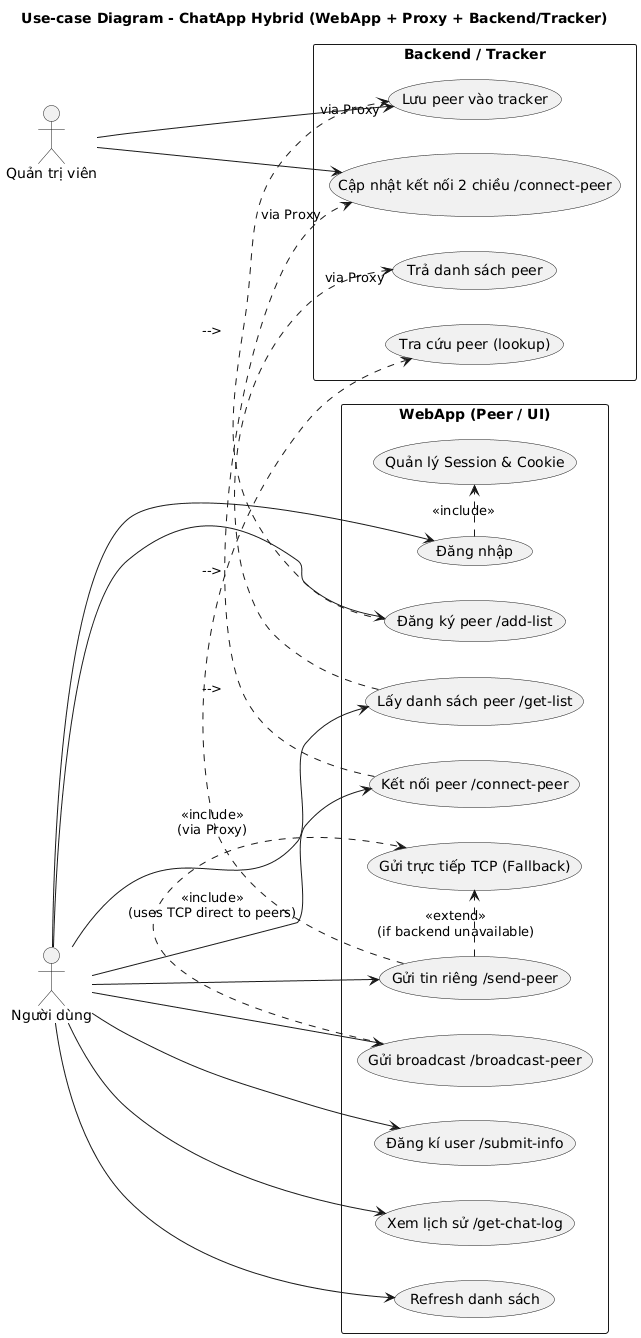
\includegraphics[width=0.5\linewidth]{picture/usecaseHeThong.png}
    \caption{Use-case Diagram}
    \label{fig:my_label}
    \end{figure}
\newpage
\subsection{Kiến trúc tổng thể}
Kiến trúc tổng thể gồm 3 phần chính:
\begin{itemize}
  \item Client–Server: giai đoạn khởi tạo và quản lý peer.
  \item Cookie \& Session: cơ chế xác thực và duy trì trạng thái người dùng.
  \item Peer-to-Peer: giai đoạn truyền thông tin trực tiếp giữa các peer.
\end{itemize}
\begin{figure}[H]
    \centering
    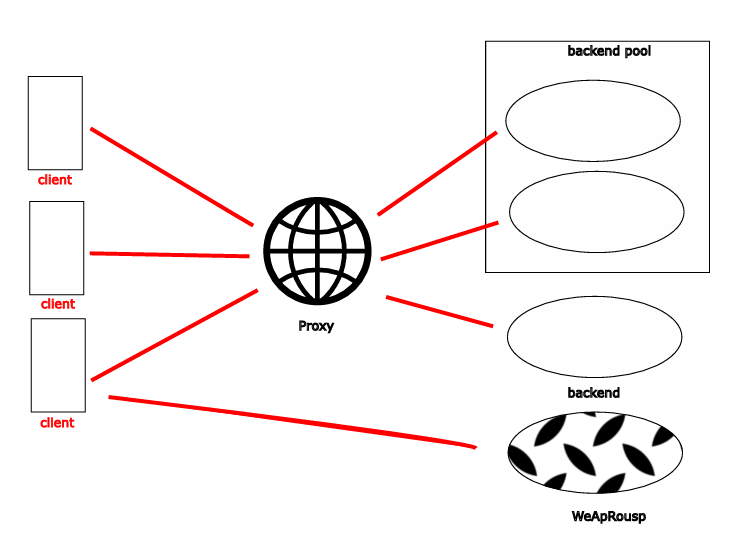
\includegraphics[width=0.5\textwidth]{picture/overview.png}
    \caption{The general view of key modules in this assignment}
    \label{fig:my_label}
\end{figure}

\textbf{Activity Diagram:}
\begin{figure}[H]
    \centering
    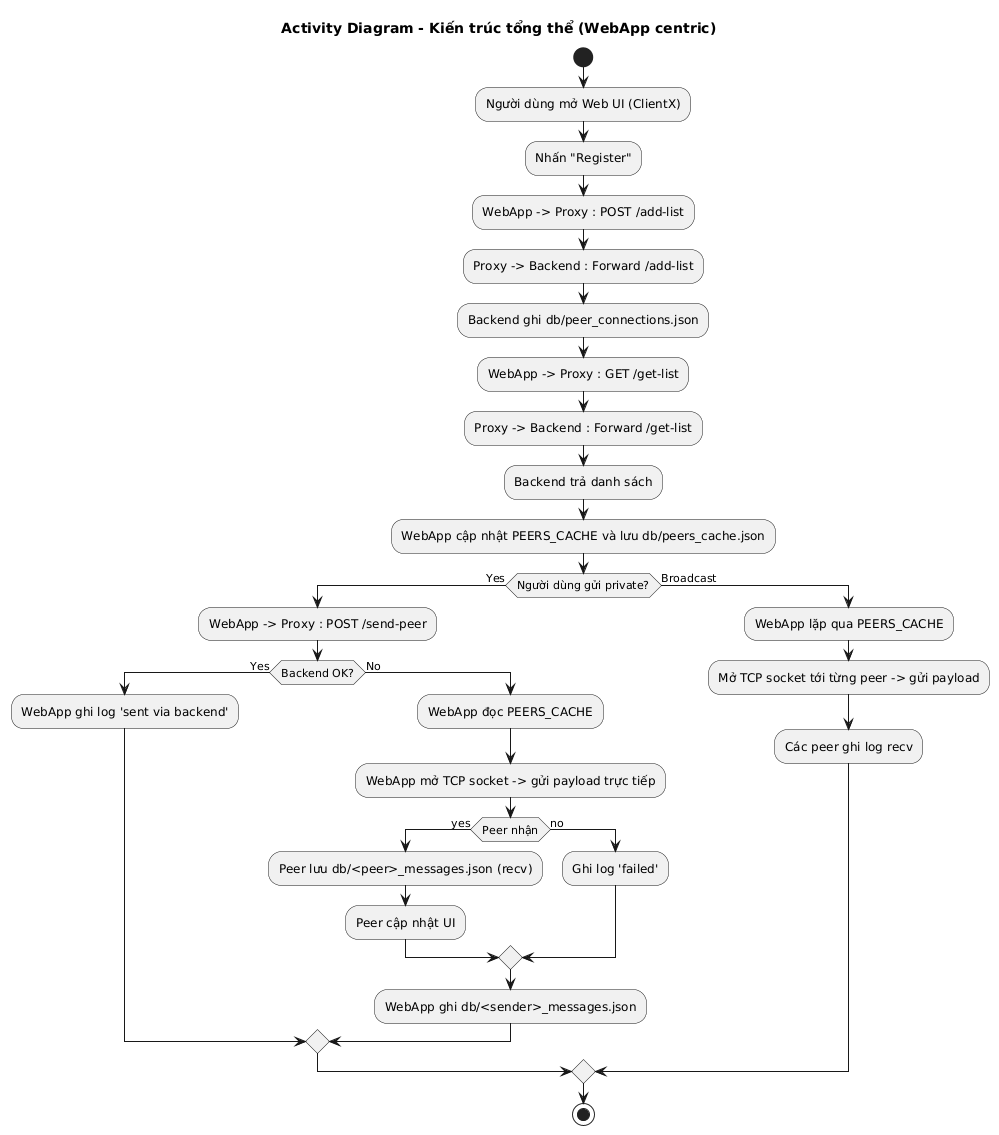
\includegraphics[width=\linewidth]{picture/activityHethong.png}
    \caption{Activity Diagram}
    \label{fig:my_label}
\end{figure}

\subsection{Thiết kế phần Client--Server}

Trong hệ thống, kiến trúc Client--Server được triển khai theo mô hình ba tầng:

\begin{itemize}
    \item \textbf{WebApp (Peer/UI):} mỗi peer (Client1, Client2, Client3) vừa đóng vai trò giao diện người dùng, vừa là tiến trình gửi các API HTTP lên backend thông qua Proxy.
    \item \textbf{Proxy (8080):} nhận mọi request từ WebApp và chuyển tiếp (forward) đến Backend dựa theo cấu hình trong \texttt{proxy.conf}.
    \item \textbf{Backend/Tracker (9000):} xử lý các API như \texttt{/add-list}, \texttt{/get-list}, \texttt{/connect-peer}, \texttt{/send-peer}, duy trì thông tin các peer trong tệp \texttt{db/peer\_connections.json}.
\end{itemize}

Luồng hoạt động Client--Server diễn ra như sau:

\begin{enumerate}
    \item Người dùng tương tác với Web UI, WebApp nhận các yêu cầu như đăng ký peer, lấy danh sách peer hoặc gửi tin nhắn.
    \item WebApp gửi HTTP request đến Proxy (127.0.0.1:8080).
    \item Proxy phân tích gói tin và forward đến Backend (127.0.0.1:9000).
    \item Backend xử lý logic ứng với từng API:
    \begin{itemize}
        \item Ghi thông tin peer vào \texttt{peer\_connections.json} khi nhận \texttt{/add-list}.
        \item Trả danh sách peer khi nhận \texttt{/get-list}.
        \item Tra cứu peer đích khi nhận \texttt{/send-peer}.
    \end{itemize}
    \item Backend trả response đến Proxy rồi về WebApp; WebApp cập nhật UI, cache và log.
\end{enumerate}

\textbf{Activity Diagram:}

\begin{figure}[H]
    \centering
    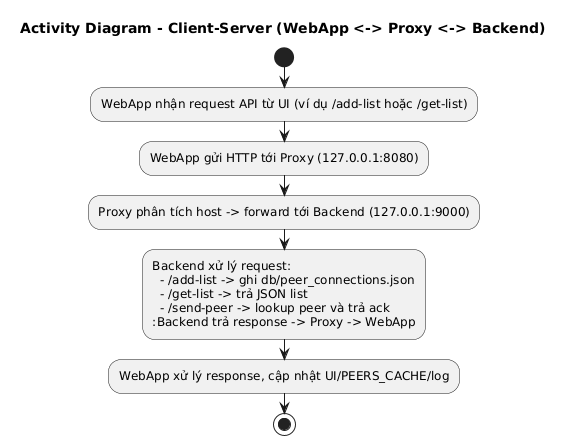
\includegraphics[width=0.8\textwidth]{picture/activityClientServer.png}
    \caption{Activity Diagram Client--Server}
\end{figure}

\subsection{Thiết kế phần Cookie \& Session}

Hệ thống sử dụng cơ chế Cookie để quản lý xác thực phiên đăng nhập. Luồng xử lý diễn ra như sau:

\begin{itemize}
    \item Người dùng gửi yêu cầu đăng nhập qua API \texttt{/login}.
    \item Backend kiểm tra thông tin người dùng trong tệp \texttt{www/users.json}.
    \item Nếu thông tin hợp lệ, backend trả về \textbf{Set-Cookie: auth=true}.
    \item Trình duyệt lưu cookie và tự động đính kèm vào các request sau.
    \item Khi người dùng truy cập các endpoint được bảo vệ như \texttt{/} hoặc \texttt{/protected}, Backend kiểm tra giá trị \texttt{req.cookies["auth"]}.
\end{itemize}

\textbf{Activity Diagram:}

\begin{figure}[H]
    \centering
    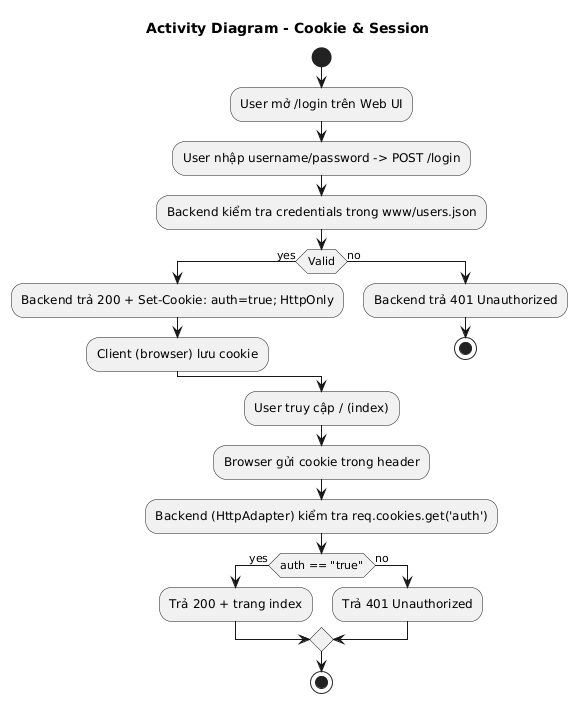
\includegraphics[width=0.7\textwidth]{picture/activityLogin.png}
    \caption{Activity Diagram Cookie \& Session}
\end{figure}

\subsection{Thiết kế phần Peer-to-Peer (P2P)}
Trong mô hình P2P của hệ thống, việc truyền tin nhắn trực tiếp giữa các peer được thực hiện bởi chính các tiến trình WebApp, không phải bởi Backend. Backend chỉ đóng vai trò \textbf{Tracker}, cung cấp thông tin peer và trả về kết quả tra cứu.

\begin{itemize}
    \item \textbf{Message Format (JSON):}
    \begin{itemize}
        \item \texttt{type}: \texttt{"private"} hoặc \texttt{"broadcast"}
        \item \texttt{sender}: tên người gửi
        \item \texttt{message}: nội dung
        \item \texttt{timestamp}: thời gian gửi
    \end{itemize}

    \item \textbf{TCP Listener:}   
    Mỗi WebApp khi khởi động sẽ tạo một TCP listener trên cổng tương ứng (9001, 9002, 9003) để nhận tin nhắn trực tiếp từ peer khác.

    \item \textbf{Luồng gửi Private Message:}
    \begin{enumerate}
        \item WebApp gửi \texttt{/send-peer} đến Backend thông qua Proxy để tra cứu IP:port của peer đích.
        \item Backend trả ACK (không gửi TCP).
        \item Nếu Backend hoạt động bình thường → WebApp ghi log và kết thúc.
        \item Nếu Backend không phản hồi → WebApp fallback sang TCP direct mode:
        \begin{itemize}
            \item đọc thông tin peer từ \texttt{PEERS\_CACHE}
            \item mở socket TCP và gửi payload JSON trực tiếp đến peer đích
        \end{itemize}
    \end{enumerate}

    \item \textbf{Luồng Broadcast:}
    WebApp lặp qua danh sách peer trong \texttt{PEERS\_CACHE}, mở socket TCP đến từng peer và gửi payload.
    
    \item \textbf{Luồng nhận:}
    WebApp đích nhận payload qua TCP, ghi log vào \texttt{db/<peer>\_messages.json} và cập nhật UI.
\end{itemize}

\textbf{Activity Diagram:}
\begin{figure}[H]
    \centering
    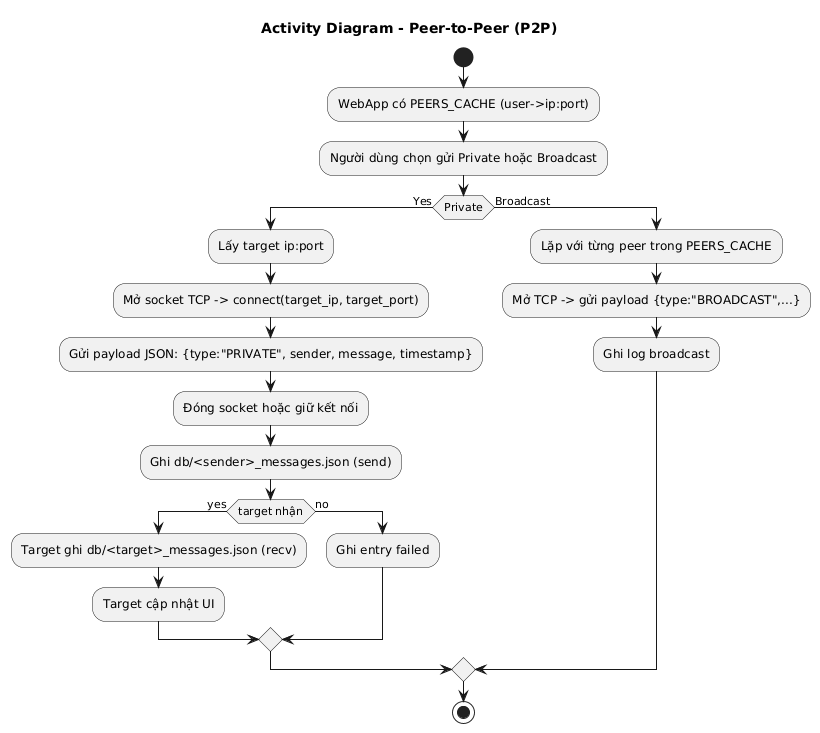
\includegraphics[width=\linewidth]{picture/activityP2Pchat.png}
    \caption{Activity Diagram}
    \label{fig:my_label}
\end{figure}
\subsection{Luồng hoạt động của hệ thống}

Luồng hoạt động tổng thể của hệ thống được triển khai theo mô hình lai (Hybrid), kết hợp giữa Client--Server và Peer--to--Peer. Các bước chính như sau:

\begin{enumerate}
    \item \textbf{Đăng nhập:}  
    Peer gửi thông tin đăng nhập, Backend xác thực bằng cookie \texttt{auth=true}.
    
    \item \textbf{Đăng ký peer:}  
    Mỗi WebApp gửi \texttt{/add-list} thông qua Proxy; Backend lưu thông tin peer vào \texttt{db/peer\_connections.json}.
    
    \item \textbf{Lấy danh sách peer:}  
    WebApp gọi \texttt{/get-list}, Backend trả về danh sách, WebApp cập nhật \texttt{PEERS\_CACHE}.
    
    \item \textbf{Gửi Private/Broadcast Message:}
    \begin{itemize}
        \item WebApp gửi \texttt{/send-peer} đến Proxy rồi đến Backend để lookup peer.
        \item Nếu Backend hoạt động thì WebApp ghi log.
        \item Nếu Backend lỗi thì WebApp fallback sang gửi TCP trực tiếp.
    \end{itemize}

\end{enumerate}

\textbf{Sequence Diagram:}

\begin{figure}[H]
    \centering
    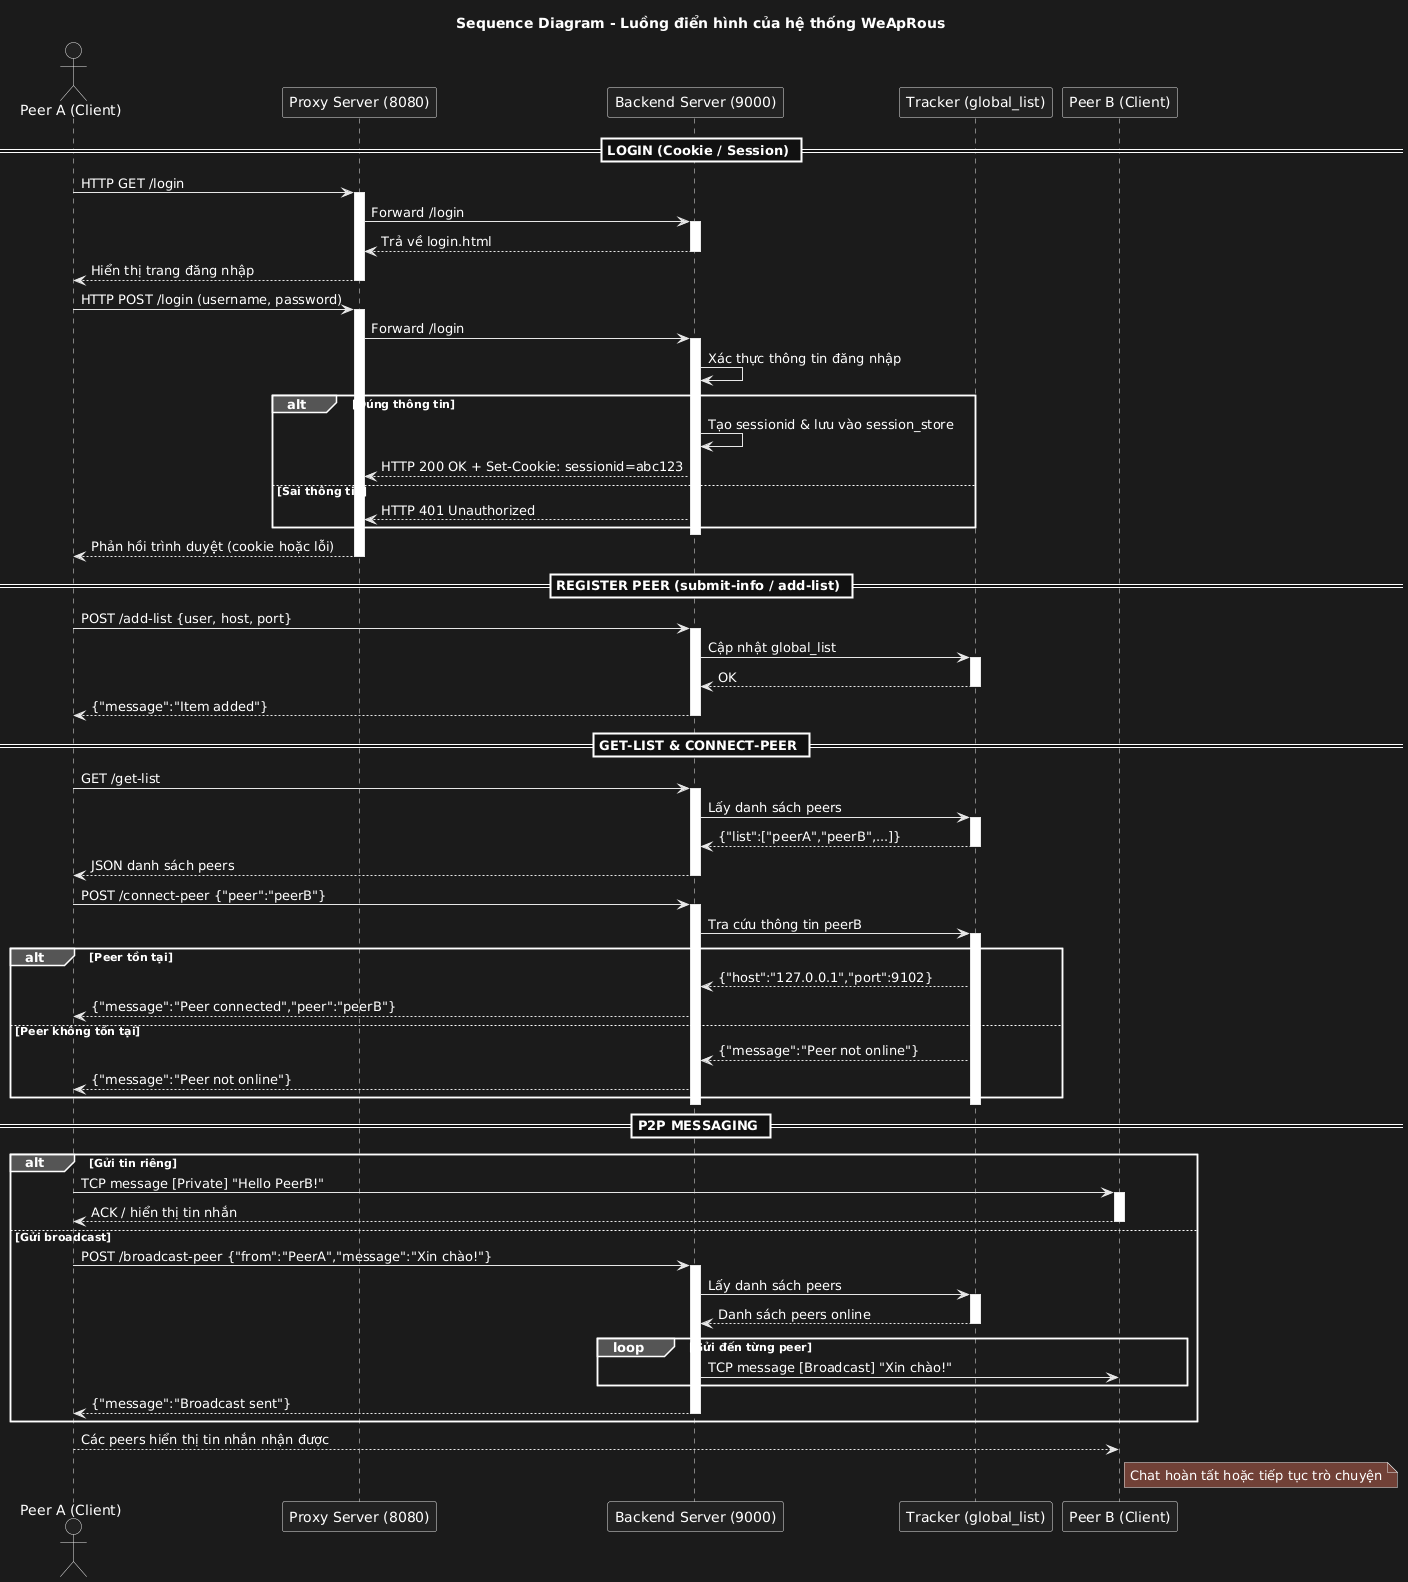
\includegraphics[width=0.9\textwidth]{picture/SequenceHeThong.png}
    \caption{Sequence Diagram toàn hệ thống}
\end{figure}

\section{Cài đặt và Kiểm thử}
\subsection{Môi trường cài đặt và khởi chạy}
Môi trường:
\begin{itemize}
    \item Python 3.13.7
    \item Các thư viện: requests, threading, socket, json
    \item Hệ điều hành: Windows 10/11
\end{itemize}

Khởi chạy:
\begin{itemize}
    \item Cài đặt server backend tại 127.0.0.1:9000  start\_backend.py --server-ip 127.0.0.1 --server-port 9000
    \item Cài đặt proxy py start\_proxy.py
\end{itemize}

\subsection{Kiểm thử chức năng đăng nhập, đăng ký}
\subsubsection{Đăng nhập}
\begin{itemize}
    \item Khi truy cập /login, nếu nhập đúng thông tin thì server trả 200 OK và đặt cookie xác thực.
    \item Nhập sai thì trả về 401 Unauthorized.
\end{itemize}
\begin{figure}[H]
    \centering
    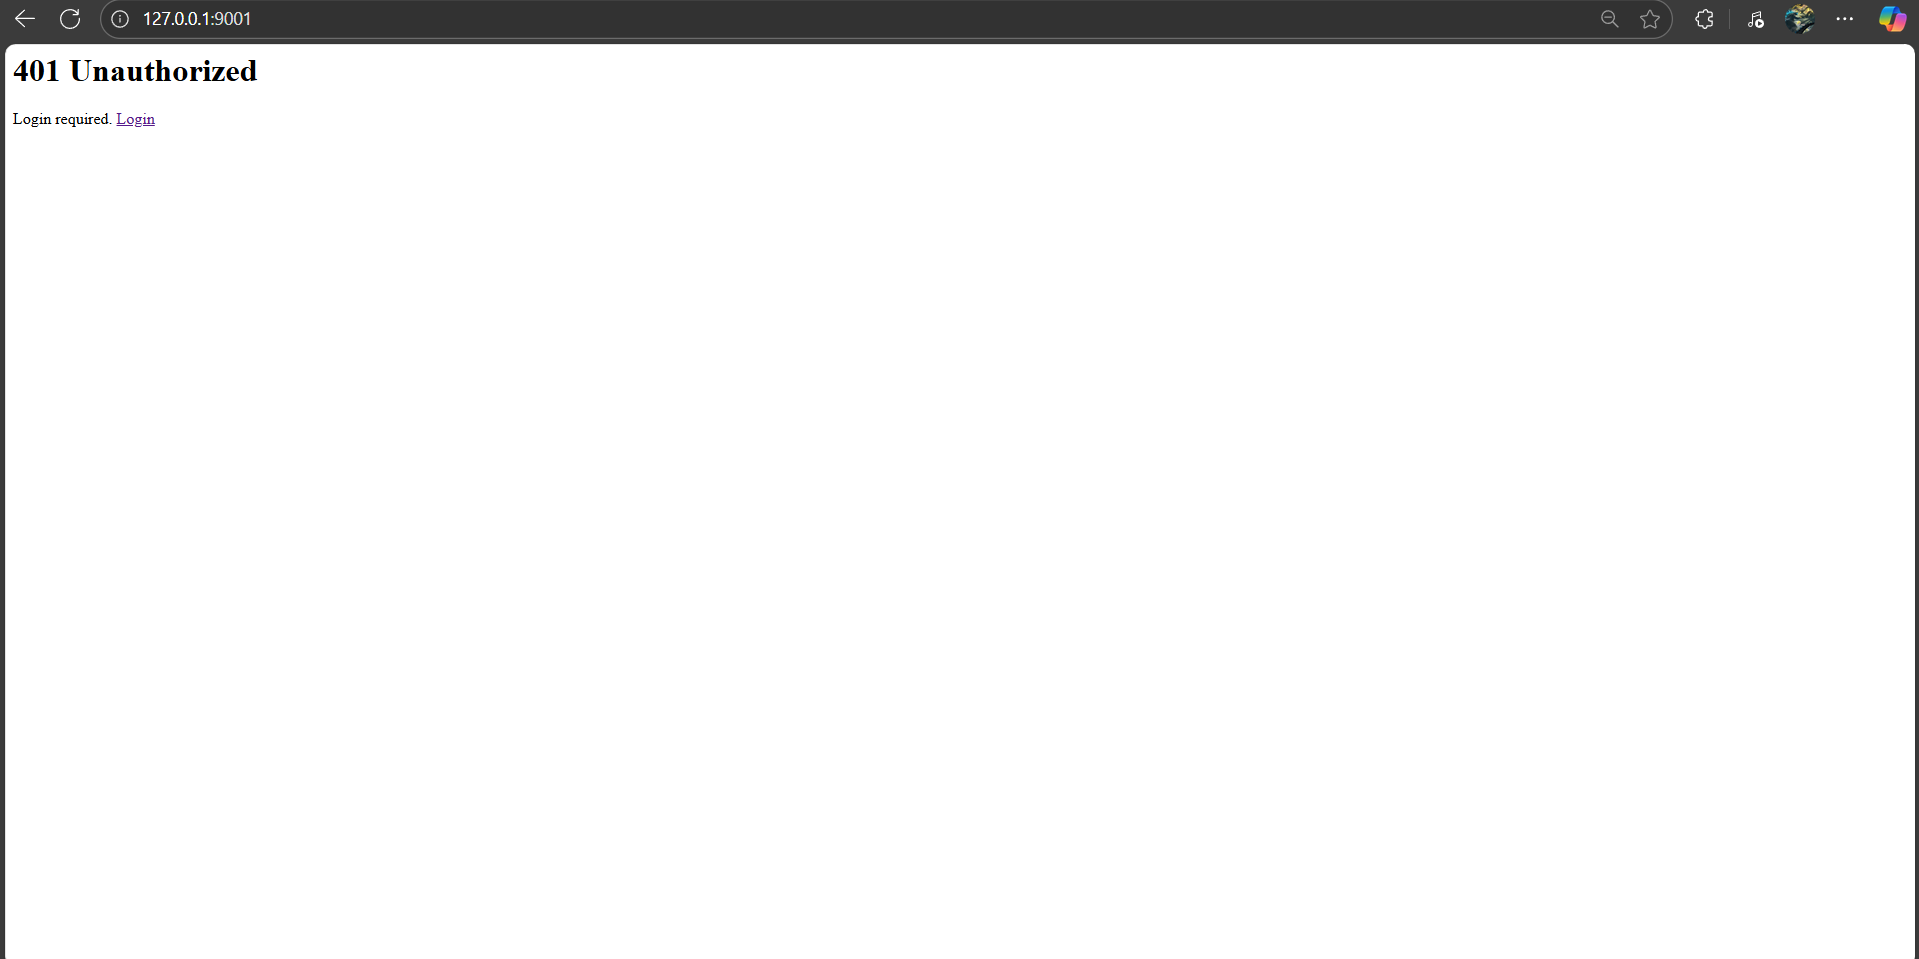
\includegraphics[width=\linewidth]{picture/chualogin.png}
    \caption{Chưa login}
    \label{fig:my_label}
\end{figure}
\begin{figure}[H]
    \centering
    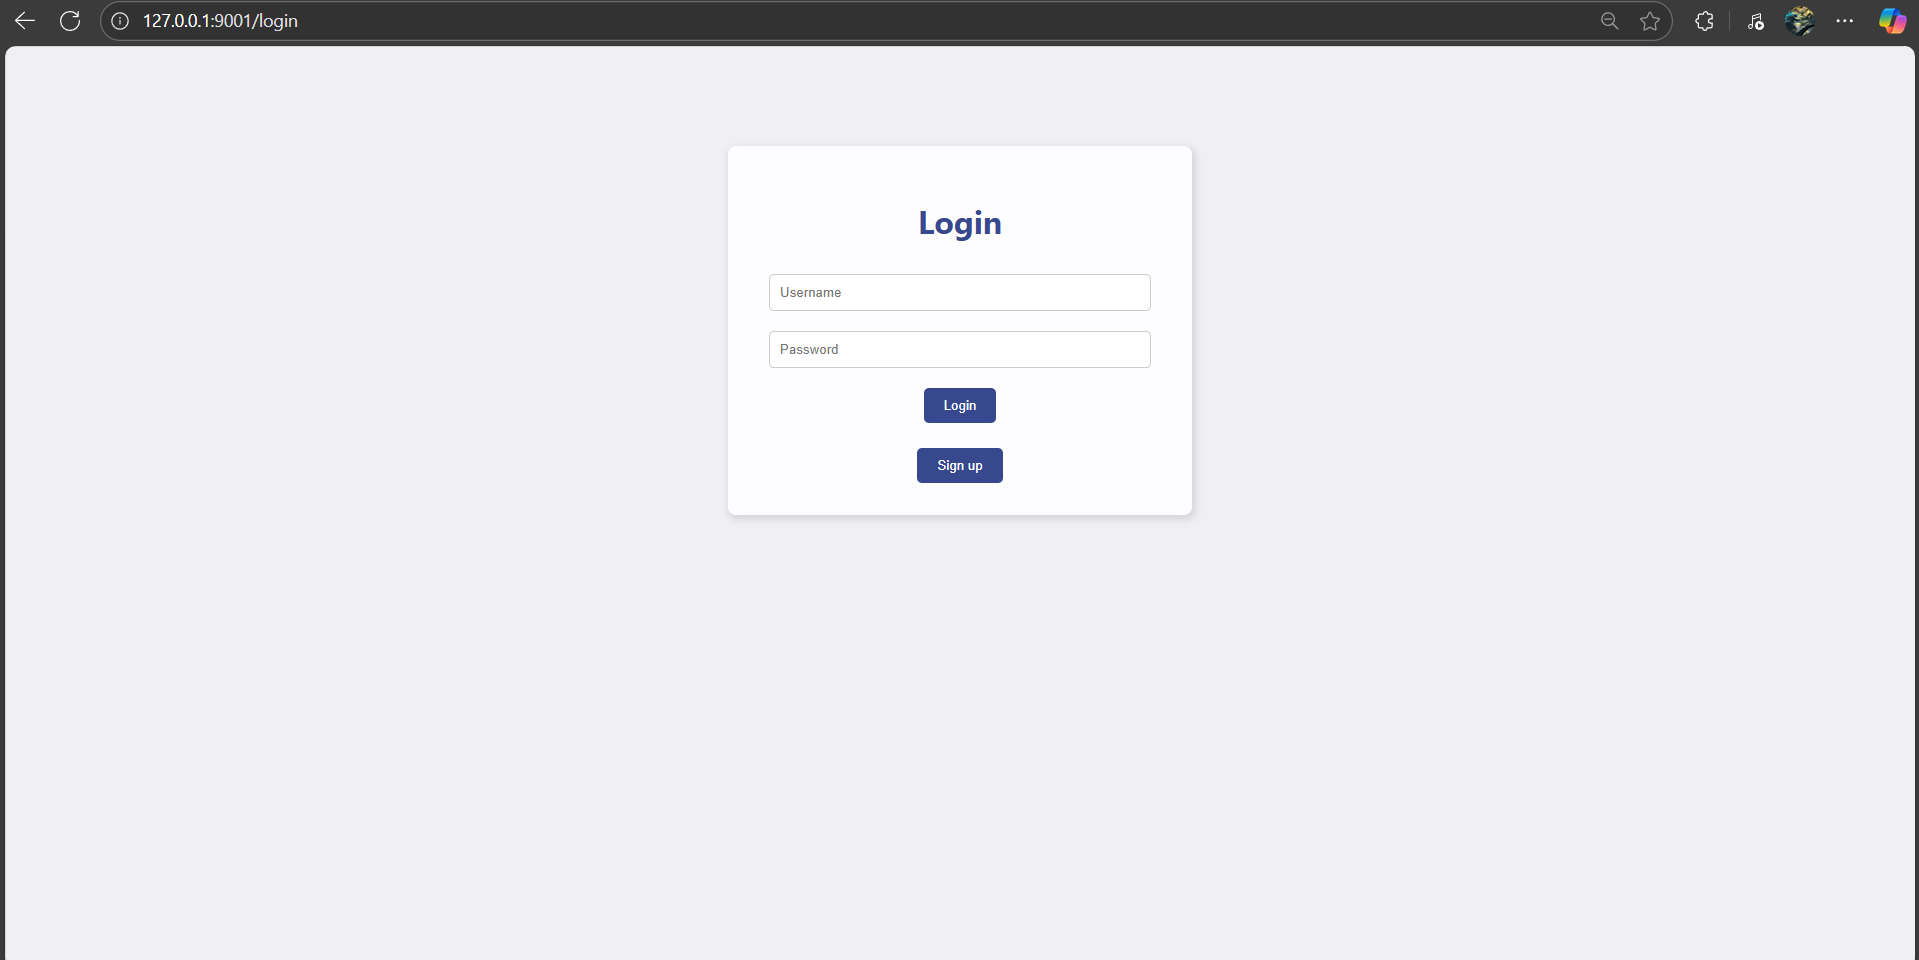
\includegraphics[width=\linewidth]{picture/login.png}
    \caption{Trang login}
    \label{fig:my_label}
\end{figure}
\begin{figure}[H]
    \centering
    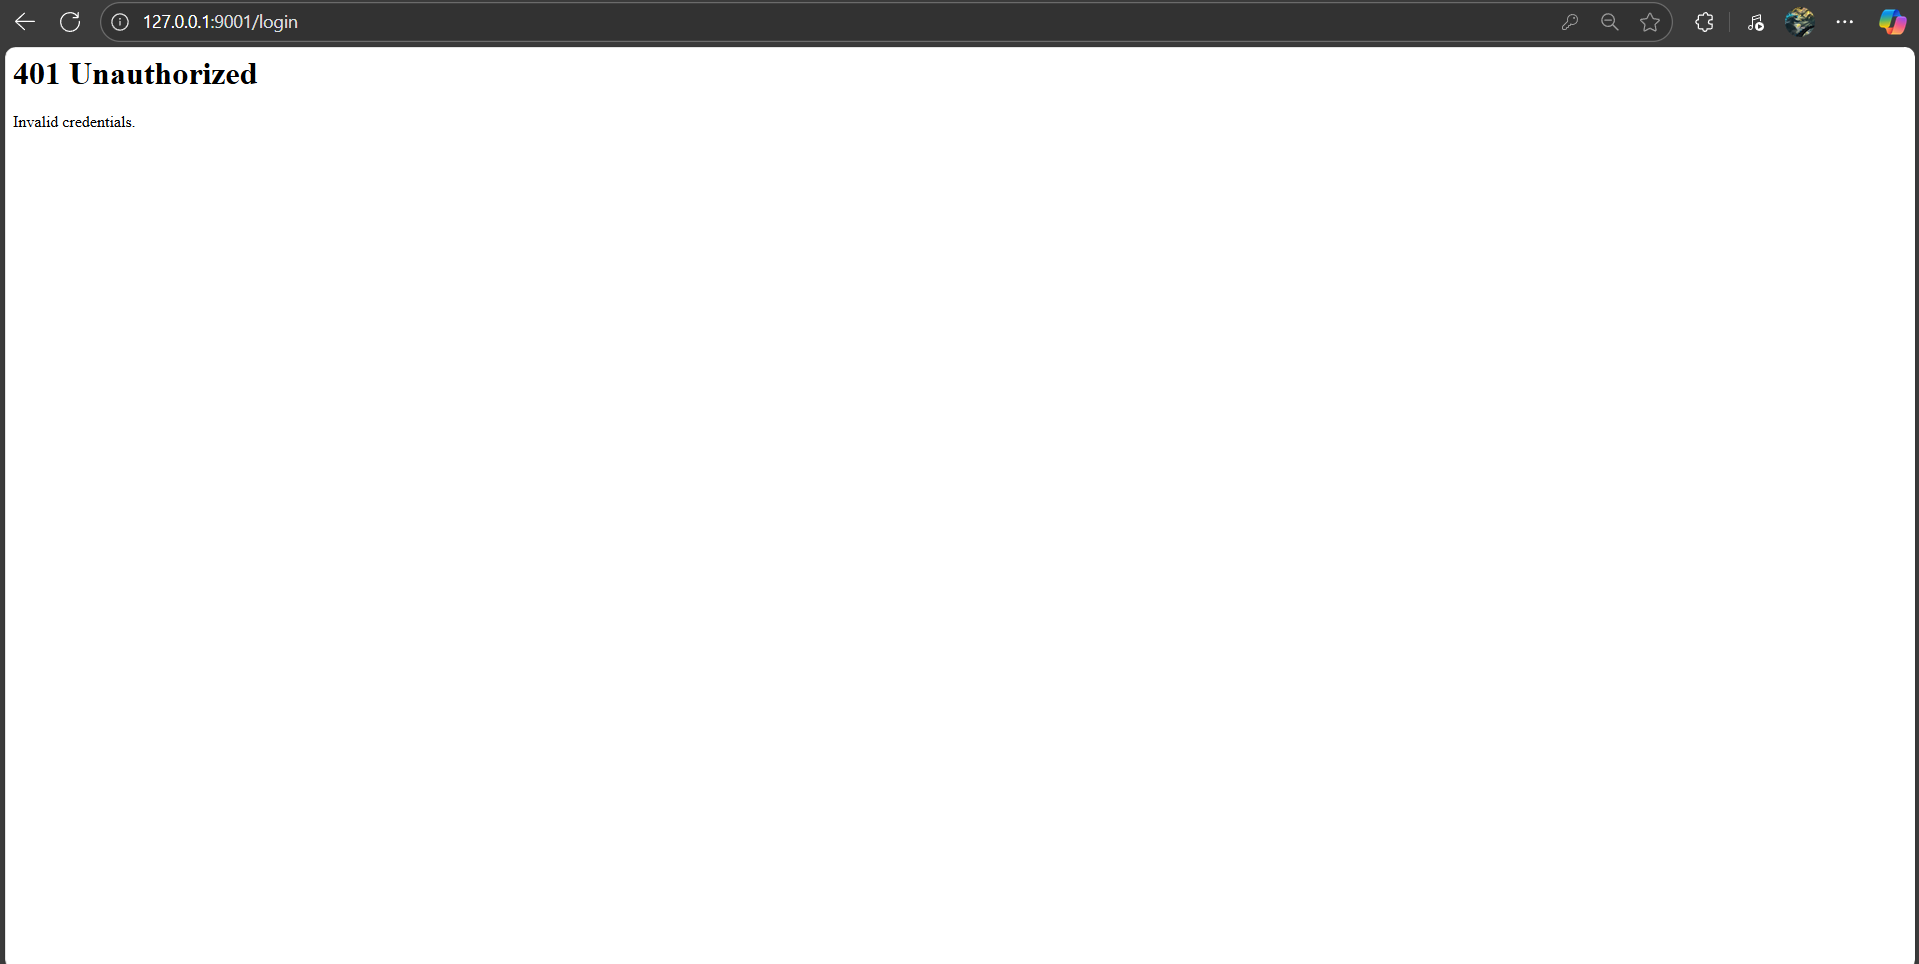
\includegraphics[width=\linewidth]{picture/kotontai.png}
    \caption{Người dùng không tồn tại}
    \label{fig:my_label}
\end{figure}
\subsubsection{đăng ký}
\begin{itemize}
    \item Gửi form /submit-info.
    \item Nếu username mới trang sẽ hiển thị “Registration Successful”.
    \item Nếu trùng username thì server trả lỗi 409 Conflict, hiển thị trên web.
    \item Sau khi đăng ký thành công, giao diện chính xác nhận người dùng đã được lưu vào users.json.
\end{itemize}
\begin{figure}[H]
    \centering
    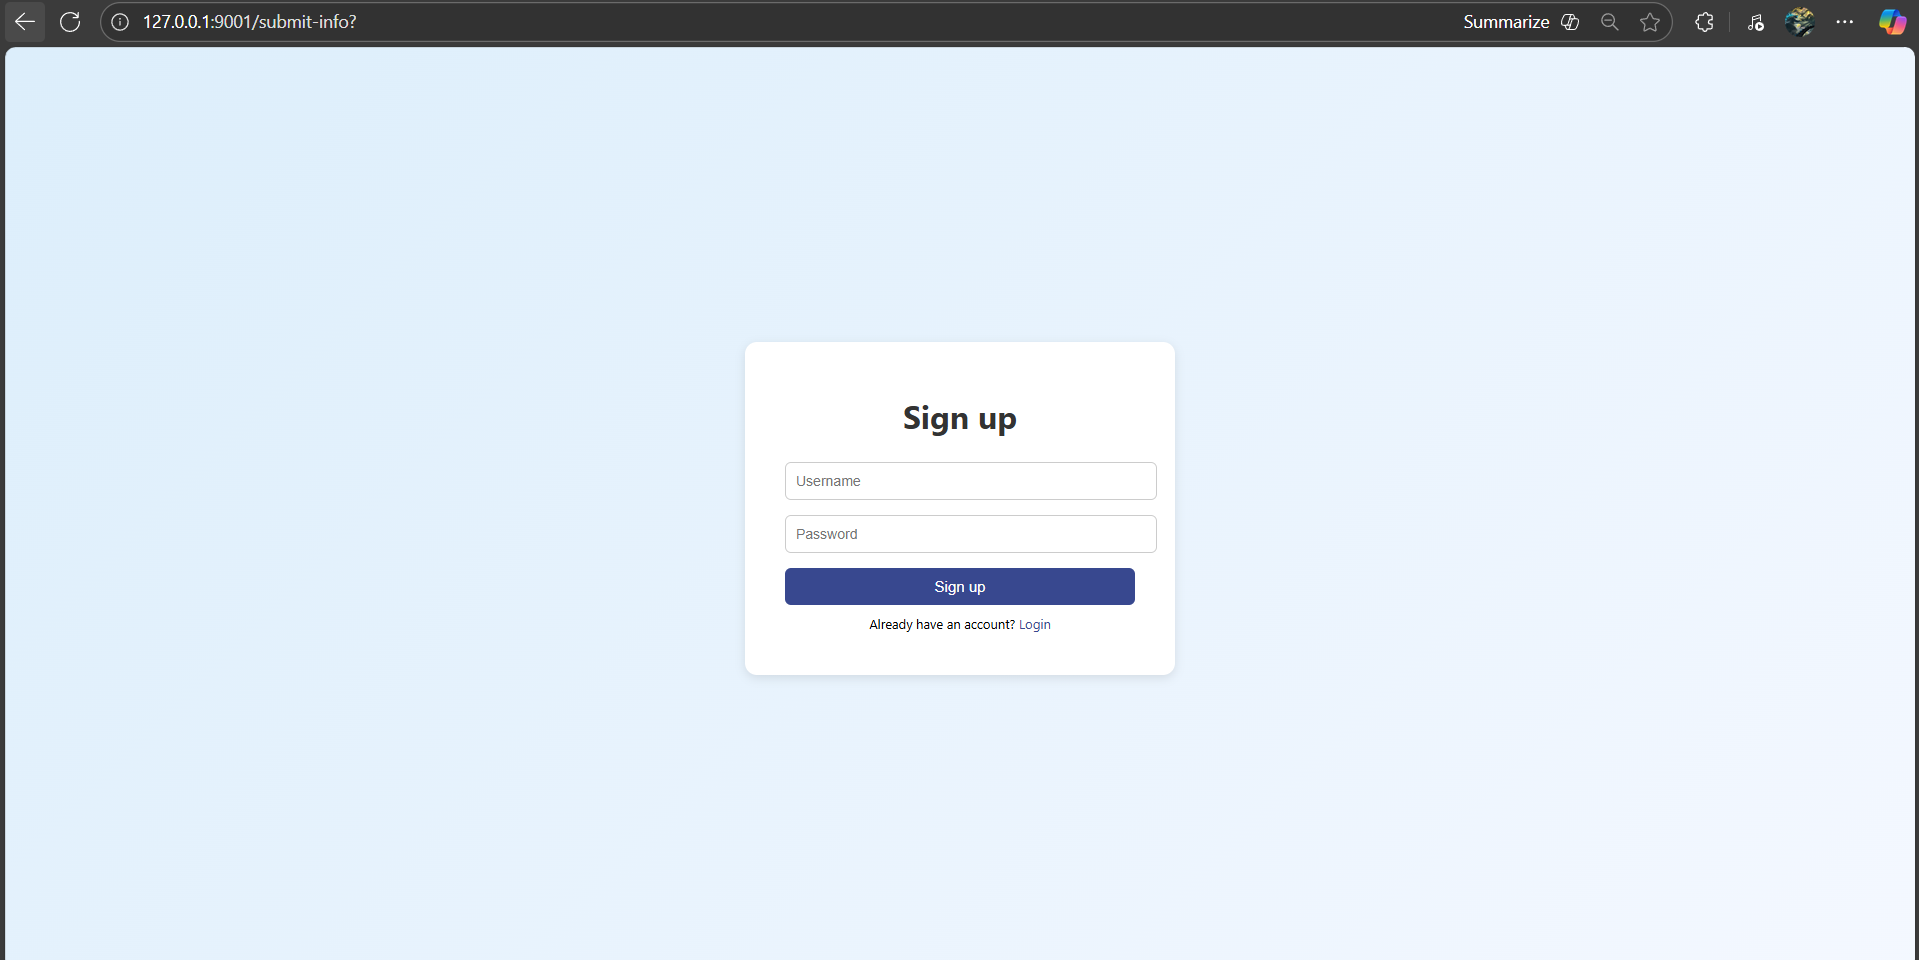
\includegraphics[width=\linewidth]{picture/dangky.png}
    \caption{Trang đăng ký}
    \label{fig:my_label}
\end{figure}
\begin{figure}[H]
    \centering
    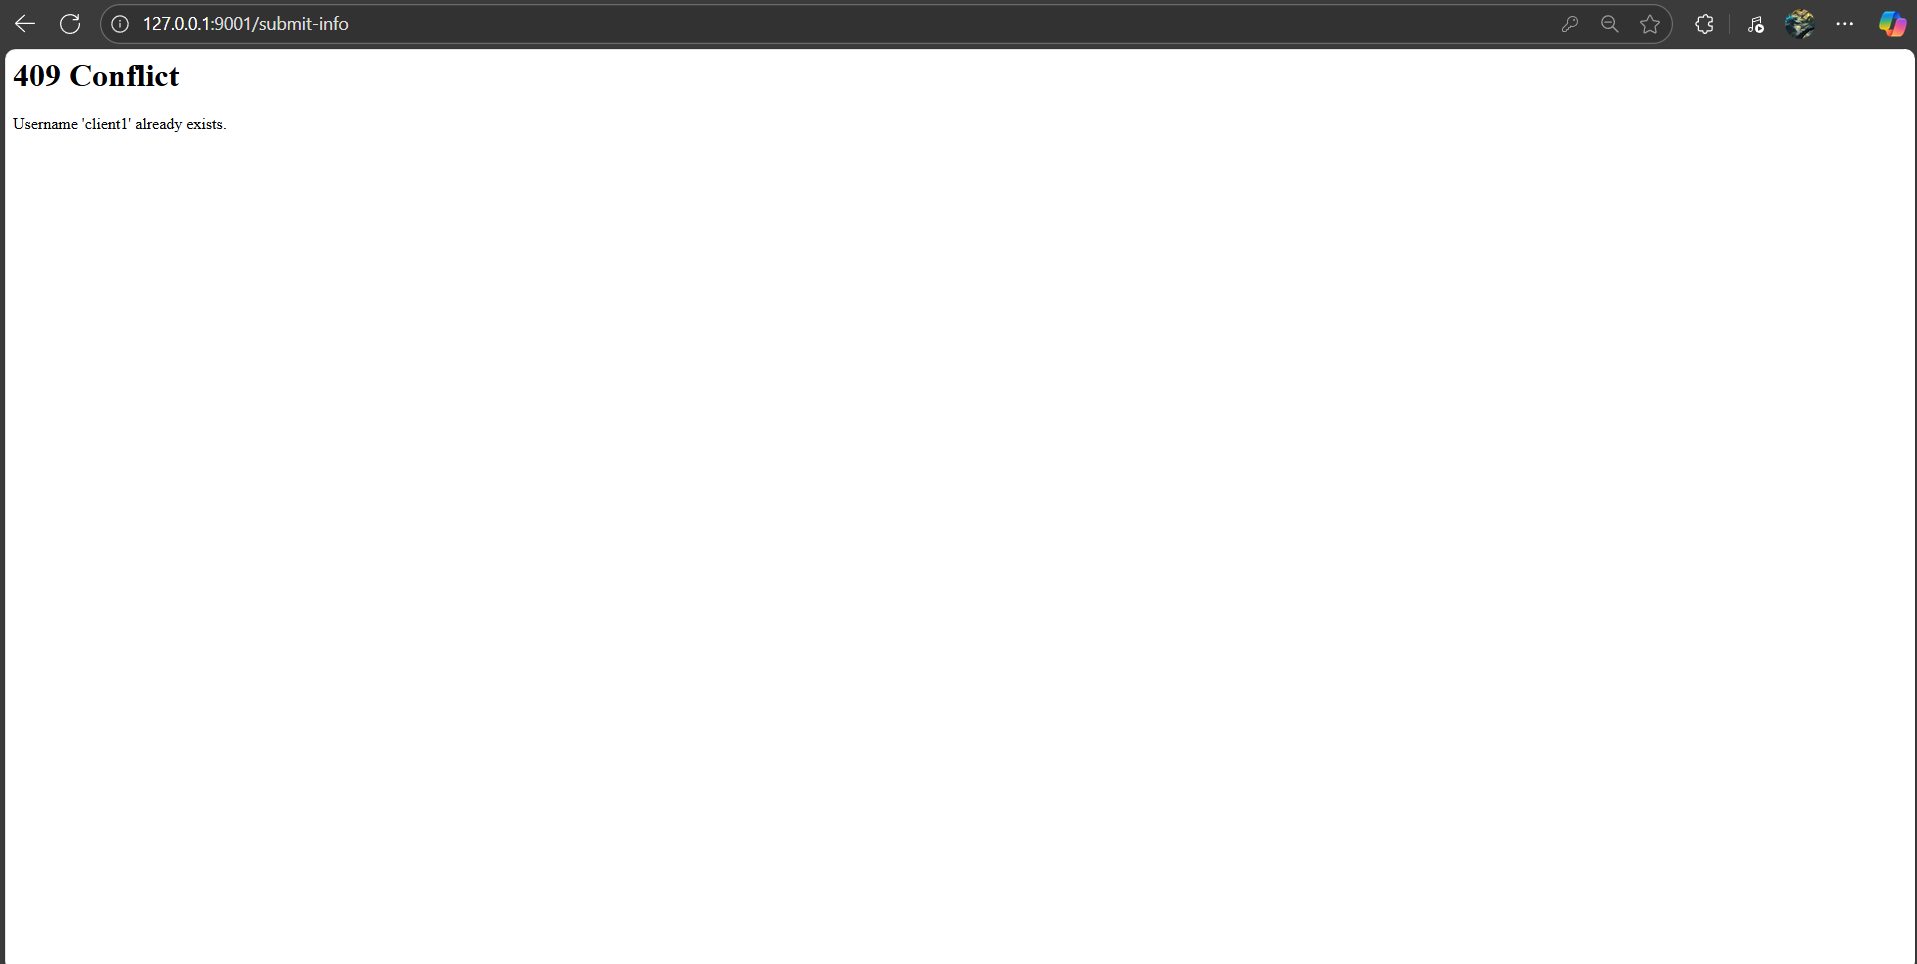
\includegraphics[width=\linewidth]{picture/trungten.png}
    \caption{Trùng tên người dùng}
    \label{fig:my_label}
\end{figure}

\begin{figure}[H]
    \centering
    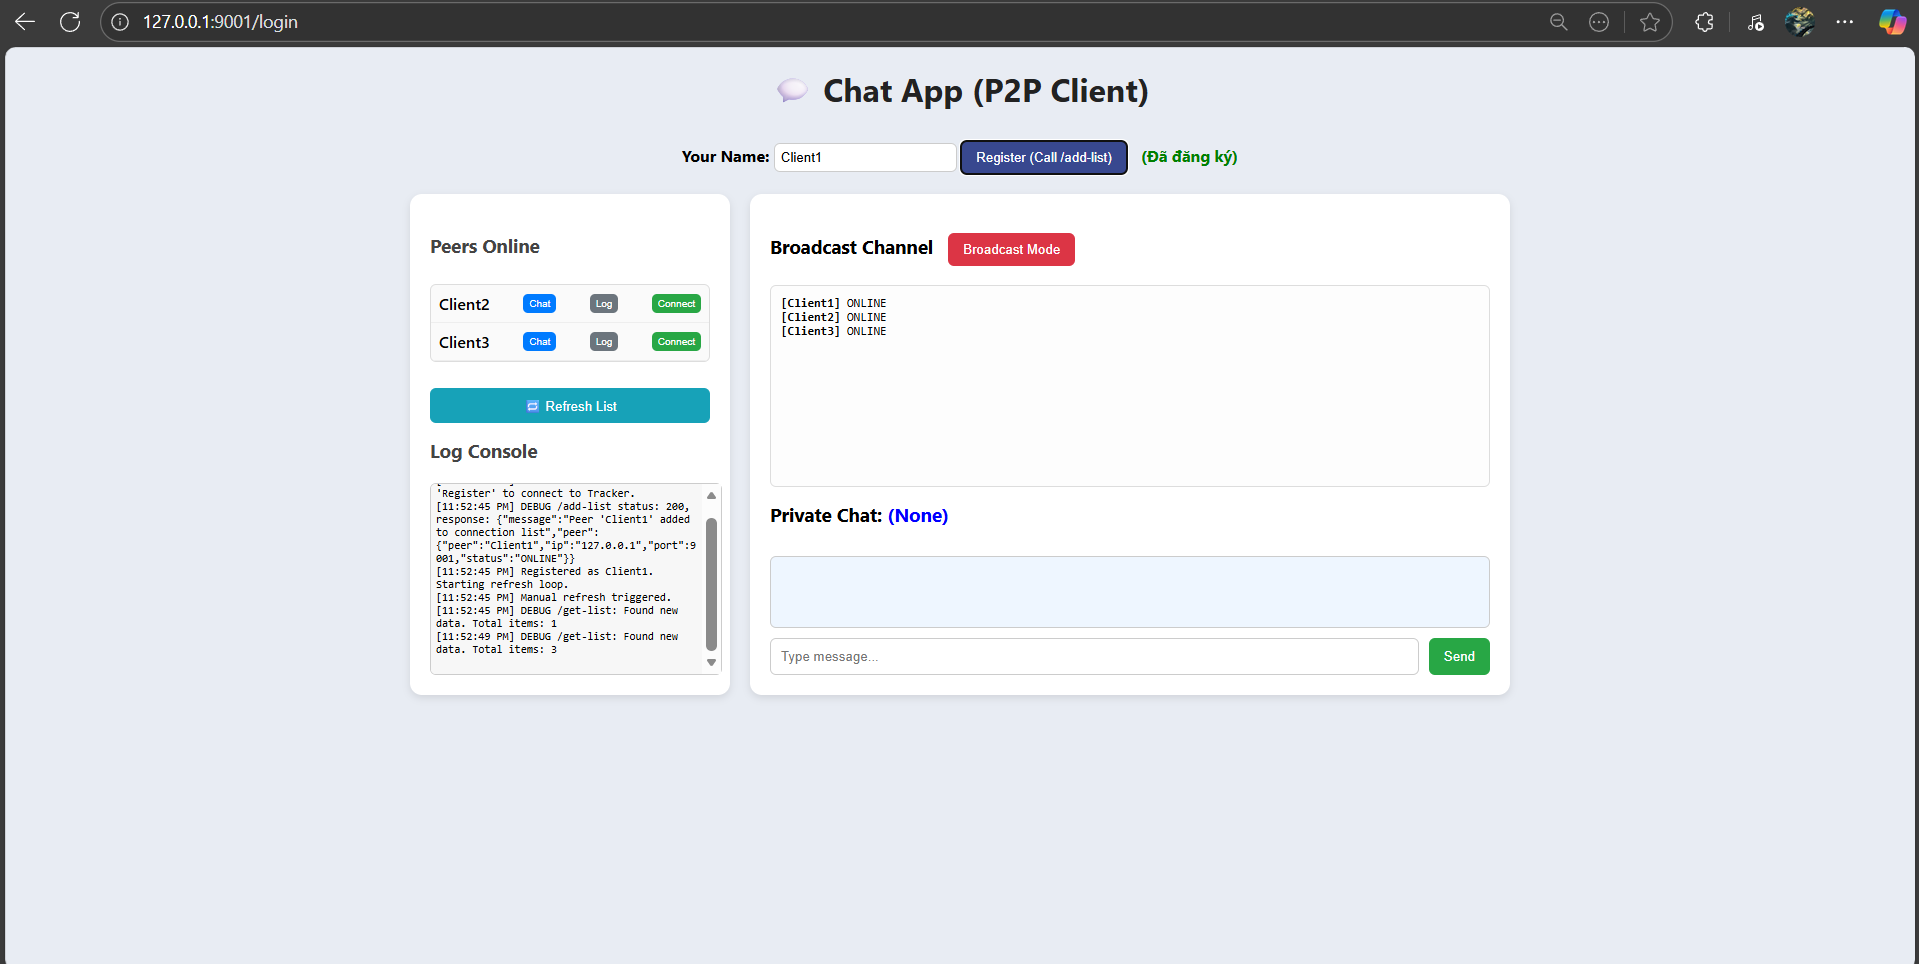
\includegraphics[width=\linewidth]{picture/UI.png}
    \caption{Giao diện chính}
    \label{fig:my_label}
\end{figure}
\subsubsection{Request Backend}
Log backend hiển thị các request liên quan đến đăng nhập (/login) và đăng ký (/submit-info).
\begin{figure}[H]
    \centering
    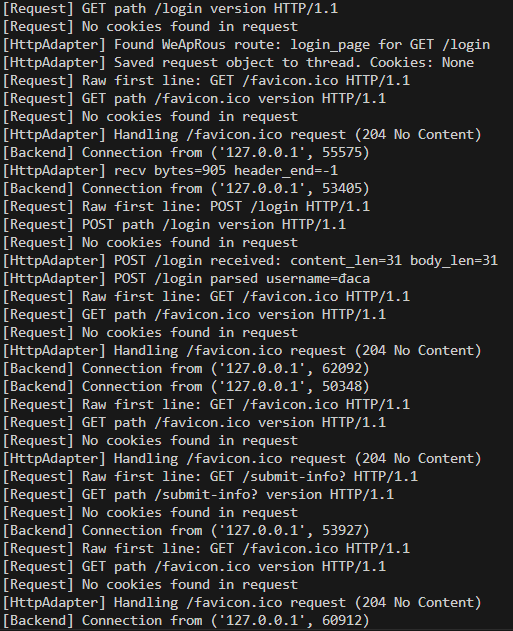
\includegraphics[width=\linewidth]{picture/backend.png}
    \caption{request backend nhận được từ các bước trên}
    \label{fig:my_label}
\end{figure}

\subsection{Kiểm thử chức năng Cookie}
Dùng test\_cookie.py để tự động gửi các request kiểm thử:
\begin{itemize}
    \item Đăng nhập hợp lệ thì sẽ trả về 200 OK và Set-Cookie: auth=true.
    \item Đăng nhập sai thì sẽ trả về 401 Unauthorized.
    \item Truy cập / mà chưa có cookie thì sẽ bị từ chối (401).
    \item Truy cập / khi có cookie hợp lệ thì sẽ thành công (200).
    \item Cookie giả mạo hoặc sai thì sẽ bị từ chối (401).
    \item Kiểm tra cô lập session giữa 2 user.
\end{itemize}

\begin{figure}[H]
    \centering
    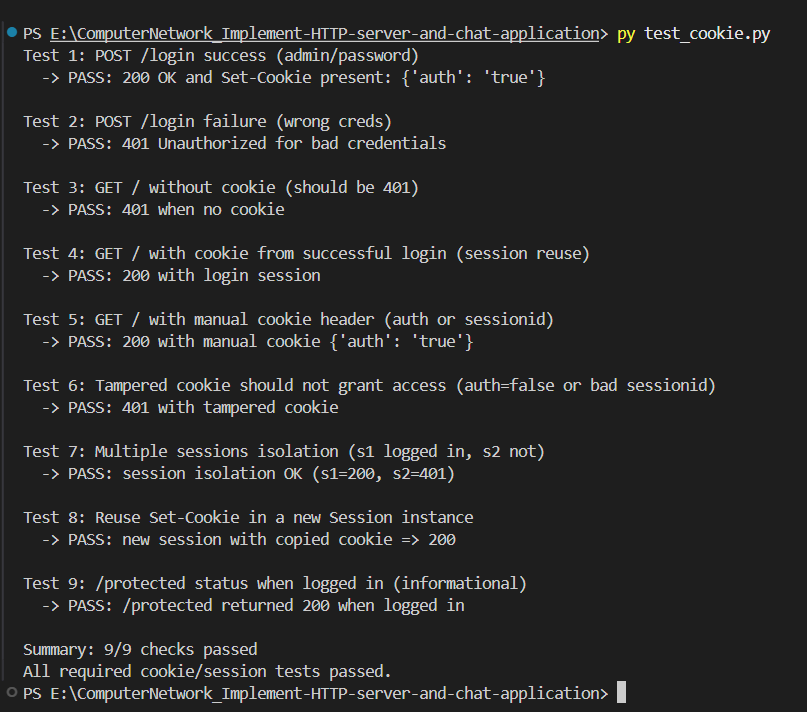
\includegraphics[width=\linewidth]{picture/test_cookie.png}
    \caption{Chạy file test\_cookie.py }
    \label{fig:my_label}
\end{figure}
\begin{figure}[H]
    \centering
    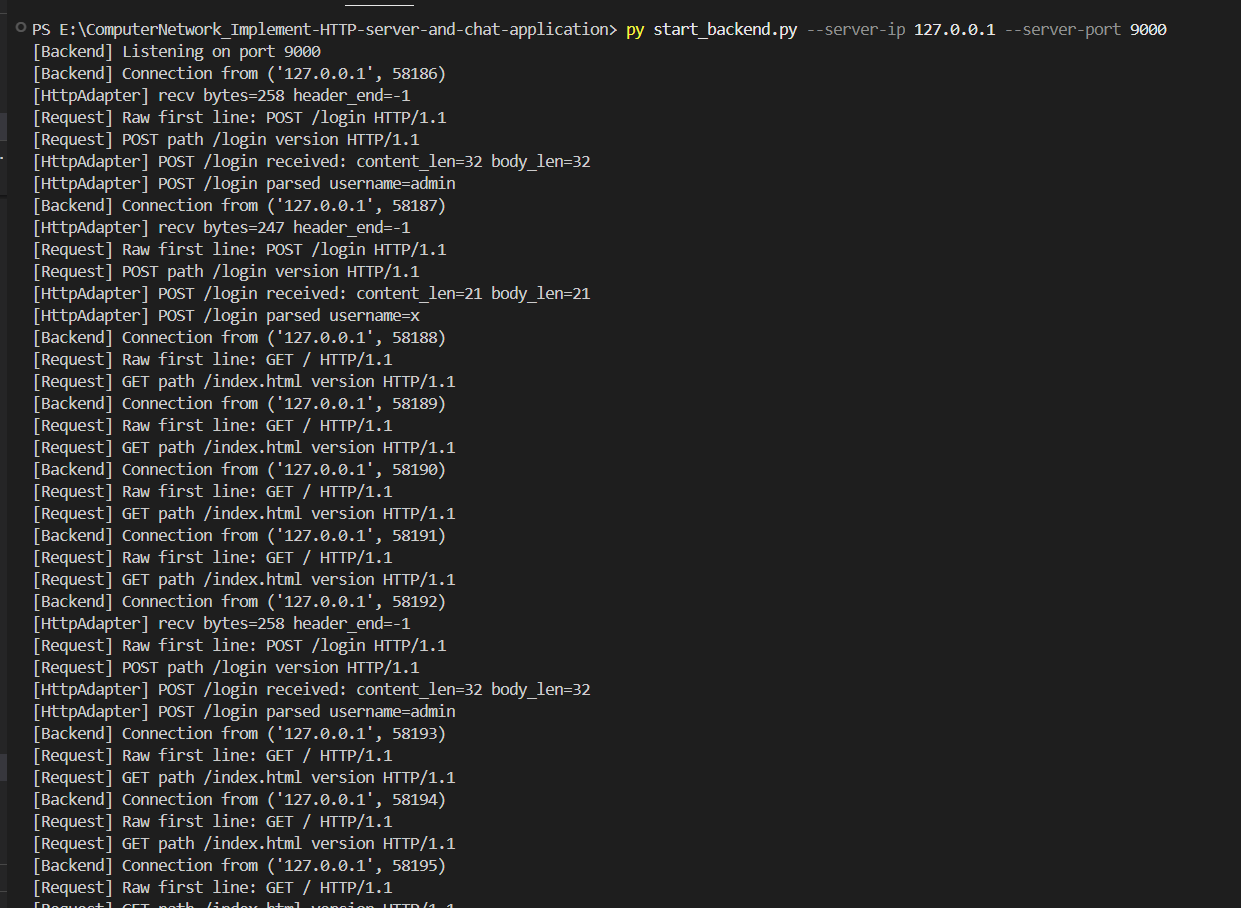
\includegraphics[width=\linewidth]{picture/backend_cookie.png}
    \caption{request backend nhận được khi chạy file test\_cookie.py}
    \label{fig:my_label}
\end{figure}
\textbf{Cookie trên Web:}
\begin{figure}[H]
    \centering
    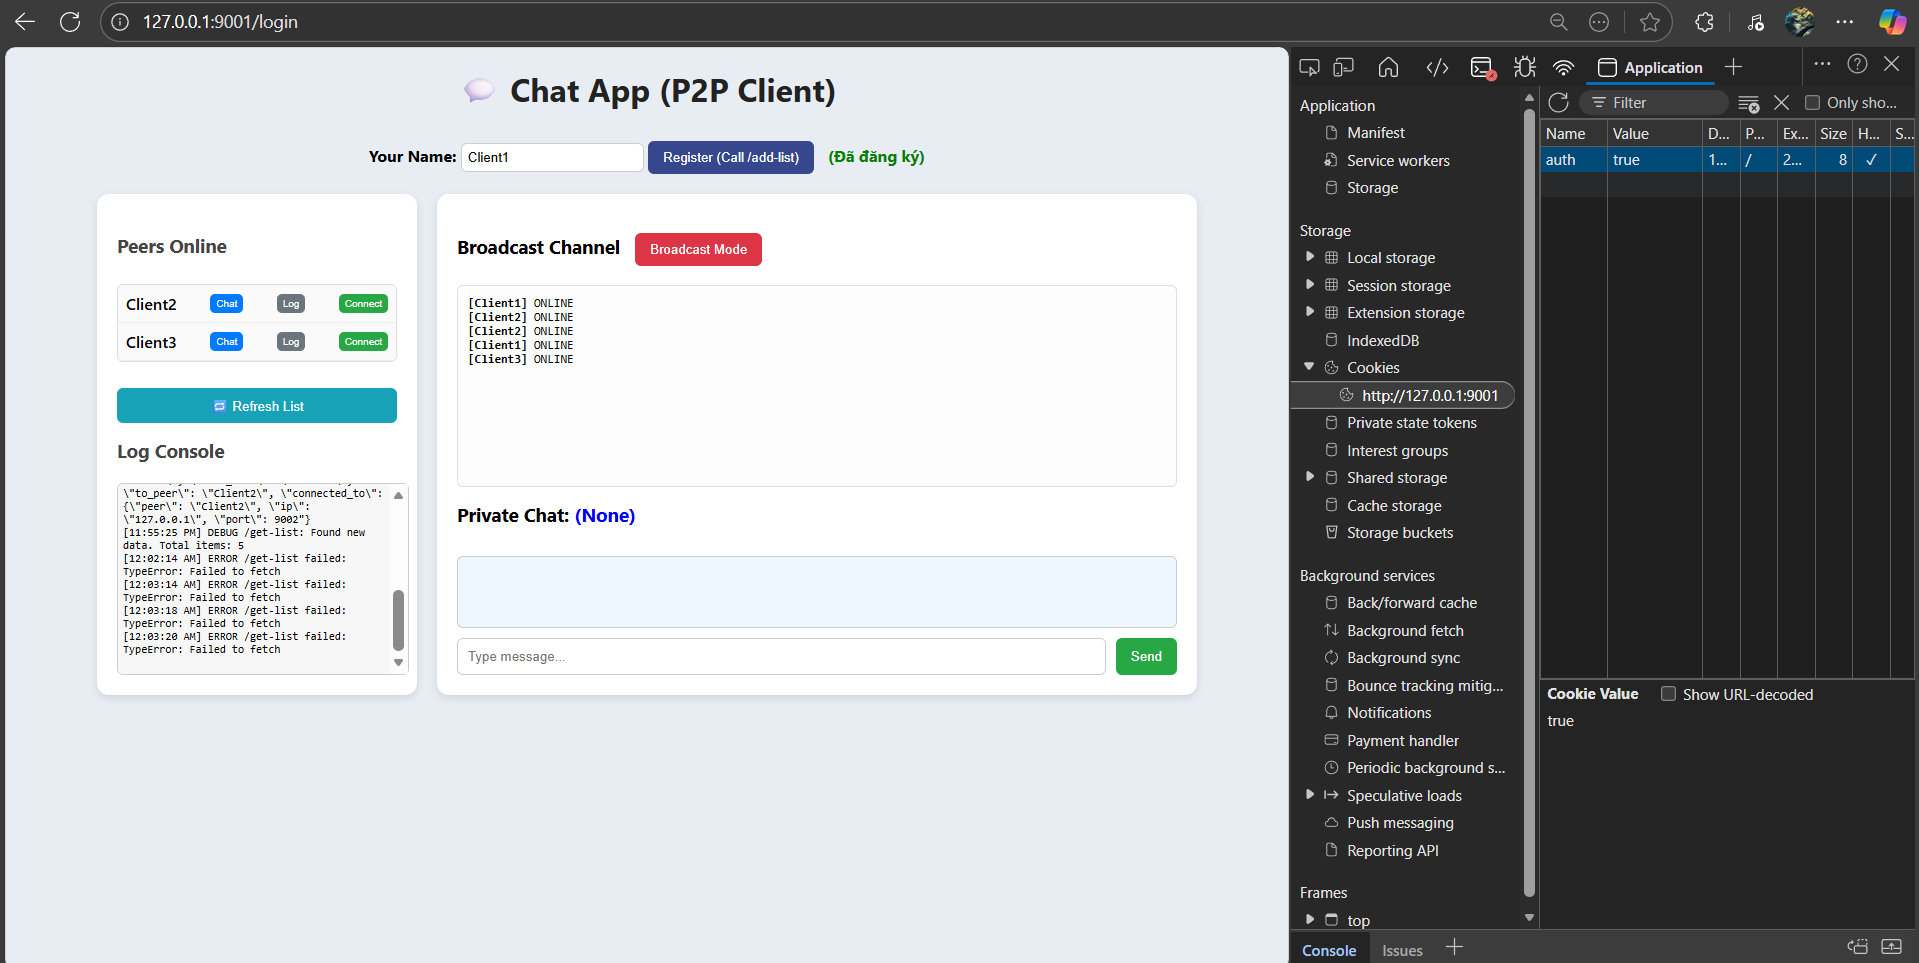
\includegraphics[width=\linewidth]{picture/cookietrue.png}
    \caption{Cookie}
    \label{fig:placeholder}
\end{figure}
\newpage
\subsection{Kiểm thử chức năng Chatapp}
Phần kiểm thử Chatapp mô phỏng mô hình lai (Hybrid Model) kết hợp giữa Client–Server và Peer-to-Peer (P2P), trong đó:
\begin{itemize}
    \item Backend (port 9000) đóng vai trò Tracker theo mô hình Client–Server, chịu trách nhiệm quản lý và lưu trữ danh sách các peer trong file \texttt{db/peer\_connections.json}.
    \item Các peer (Client1, Client2, Client3) là các tiến trình WebApp chạy ở các cổng khác nhau (ví dụ 9001/9002/9003); các peer có thể giao tiếp trực tiếp qua socket TCP theo mô hình P2P (fallback hoặc broadcast).
    \item Proxy (port 8080) hoạt động như lớp trung gian: WebApp forward mọi API tới \texttt{http://127.0.0.1:8080} và Proxy sẽ route và forward request tới Backend (127.0.0.1:9000) dựa theo \texttt{proxy.conf}.
    \item Mọi sự kiện chat được ghi nhận cục bộ trong các file log: \texttt{db/<peer>\_messages.json} (ghi các mục \texttt{send}, \texttt{recv}, \texttt{failed}, ...).
\end{itemize}

Mục tiêu của kiểm thử là chứng minh rằng hệ thống có thể:
\begin{itemize}
    \item Đăng ký peer thành công lên Backend thông qua API \texttt{/add-list} (flow: WebApp đến Proxy(8080) đến Backend(9000)) và Backend lưu mục nhập vào \texttt{db/peer\_connections.json}.
    \item Duy trì và trả về danh sách các peer đang hoạt động qua API \texttt{/get-list}; WebApp cập nhật \texttt{PEERS\_CACHE} và lưu sang \texttt{db/peers\_cache.json}.
    \item Gửi và nhận tin nhắn P2P thành công thông qua API \texttt{/send-peer} và trong trường hợp Backend không khả dụng WebApp sẽ fallback gửi TCP trực tiếp tới IP:port của peer, đồng thời log các sự kiện gửi/nhận vào file tương ứng.
\end{itemize}

\textbf{Chạy Client (WebApp) — Client1, Client2, Client3:}\\
Client1, Client2, Client3 là ba tiến trình WebApp độc lập chạy song song (ví dụ cổng 9001, 9002, 9003). Mỗi peer khởi động kèm một TCP listener để nhận kết nối P2P khi cần; đồng thời cung cấp giao diện Web UI để người dùng thao tác.

Khi khởi động, mỗi peer (WebApp) thực hiện tuần tự:
\begin{itemize}
    \item Gọi \texttt{POST /add-list} tới WebApp local (ví dụ \texttt{http://127.0.0.1:9001/add-list})  — WebApp sẽ forward request tới Proxy \texttt{127.0.0.1:8080} và Proxy forward tới Backend \texttt{127.0.0.1:9000} để đăng ký thông tin \texttt{user, host, port} trong \texttt{db/peer\_connections.json}.
    \item Gọi \texttt{GET /get-list} để nhận danh sách các peer đang online; WebApp cập nhật bộ nhớ đệm \texttt{PEERS\_CACHE} và lưu sang \texttt{db/peers\_cache.json}.
    \item Sau khi có danh sách, người dùng có thể thao tác qua Web UI để thực hiện \texttt{/connect-peer}, \texttt{/send-peer} hoặc \texttt{/broadcast-peer}.
\end{itemize}

\textbf{Backend (Tracker) — cổng 9000:}
\begin{itemize}
    \item Backend hoạt động như \textbf{tracker}: nhận các API \texttt{/add-list}, \texttt{/get-list}, \texttt{/connect-peer}, \texttt{/send-peer}, \texttt{/broadcast-peer} và cập nhật/tra cứu file \texttt{db/peer\_connections.json}.
    \item Backend chịu trách nhiệm \textbf{điều phối và khám phá peer} (không phải là media relay). Trong code hiện tại, backend trả kết quả xác nhận cho các API; việc gửi dữ liệu TCP trực tiếp có thể do WebApp thực hiện (fallback hoặc logic gửi trực tiếp).
    \item Log backend in ra console cho thấy việc nhận request và ghi file tracker, chứng minh quá trình đăng ký và lấy danh sách hoạt động chính xác.
\end{itemize}
\begin{figure}[H]
    \centering
    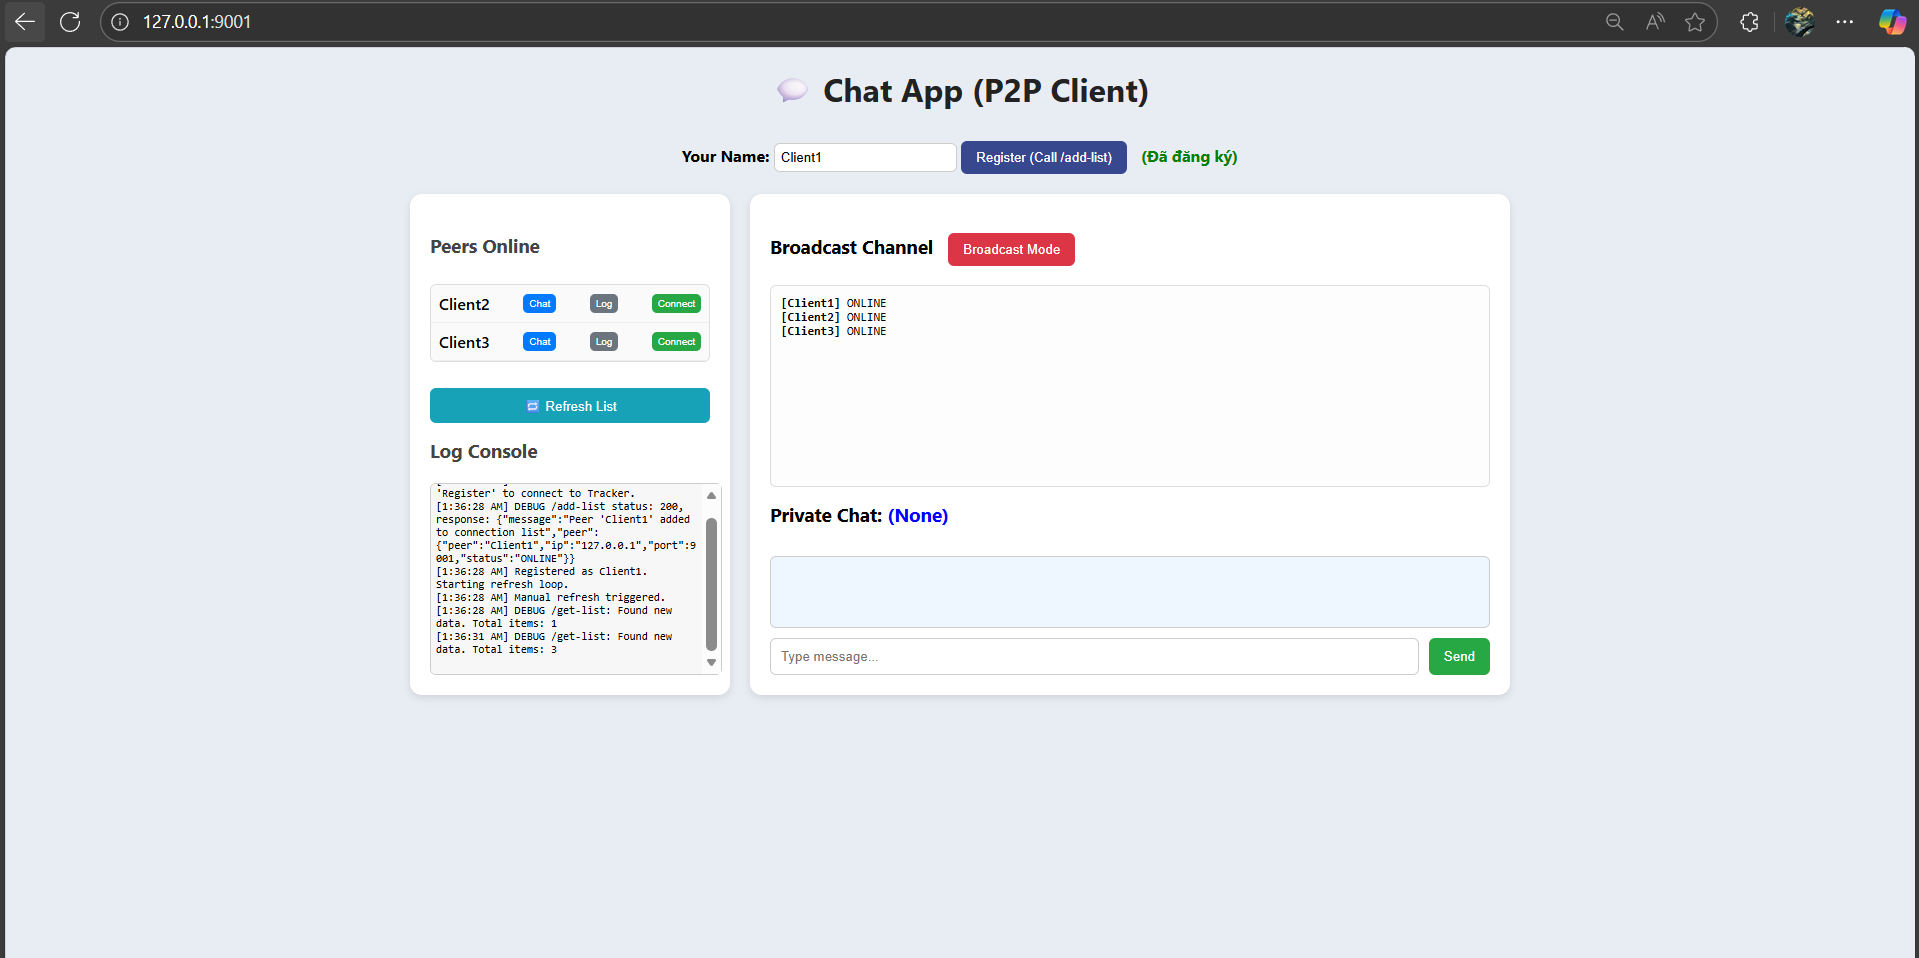
\includegraphics[width=\linewidth]{picture/UIclient1.png}
    \caption{Add-list Client1}
    \label{fig:placeholder}
\end{figure}
\begin{figure}[H]
    \centering
    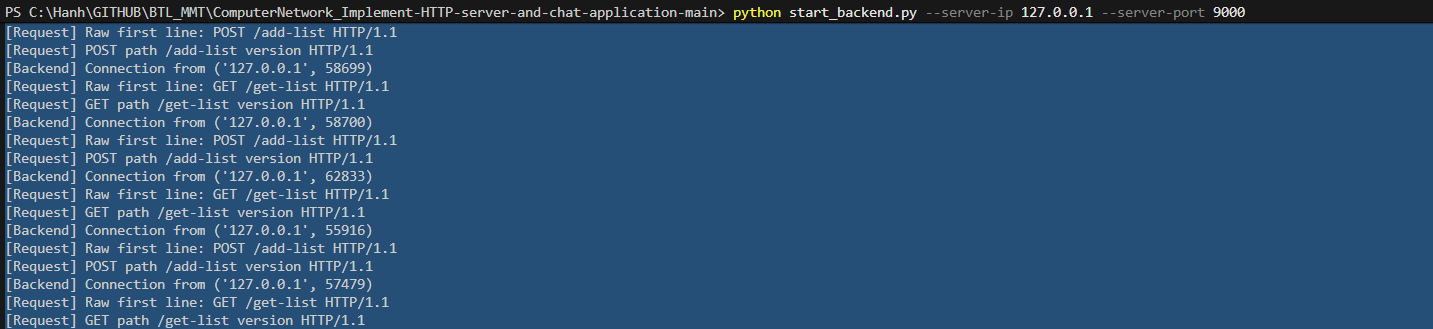
\includegraphics[width=\linewidth]{picture/backend_addlist.png}
    \caption{Backend nhận add-list}
    \label{fig:placeholder}
\end{figure}
\begin{figure}[H]
    \centering
    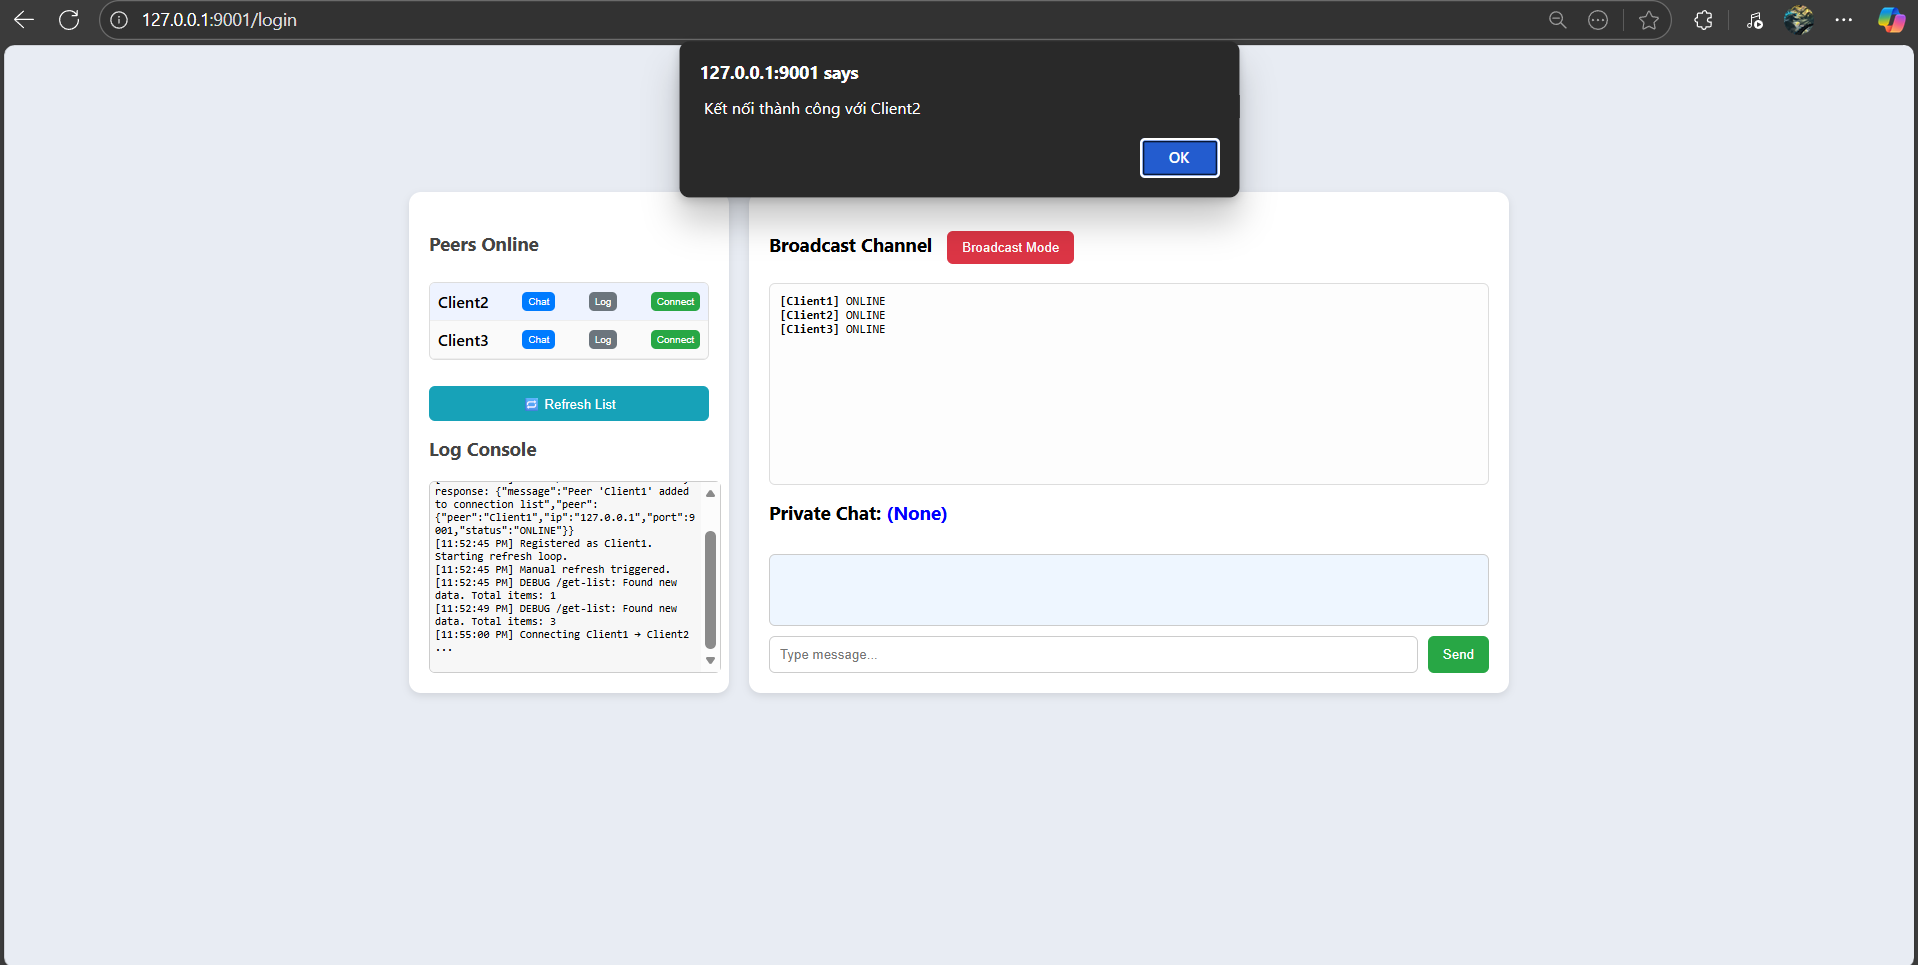
\includegraphics[width=\linewidth]{picture/connectpeer.png}
    \caption{Connect Client1 và Client2}
    \label{fig:placeholder}
\end{figure}
\textbf{Proxy (Reverse proxy) — cổng 8080:}
\begin{itemize}
    \item Proxy nhận mọi request từ WebApp (cấu hình WebApp: \texttt{BACKEND\_URL = "http://127.0.0.1:8080"}) và forward tới backend 9000 dựa theo \texttt{proxy.conf}.
    \item Proxy mô phỏng gateway trong môi trường thực: che giấu địa chỉ backend, tập trung truy cập qua một cổng duy nhất và hỗ trợ ánh xạ nhiều host/domain.
    \item Log proxy minh họa việc forward: ví dụ: \texttt{[Proxy] Host name 127.0.0.1:8080 is forwarded to 127.0.0.1:9000}.
\end{itemize}
\begin{figure}[H]
    \centering
    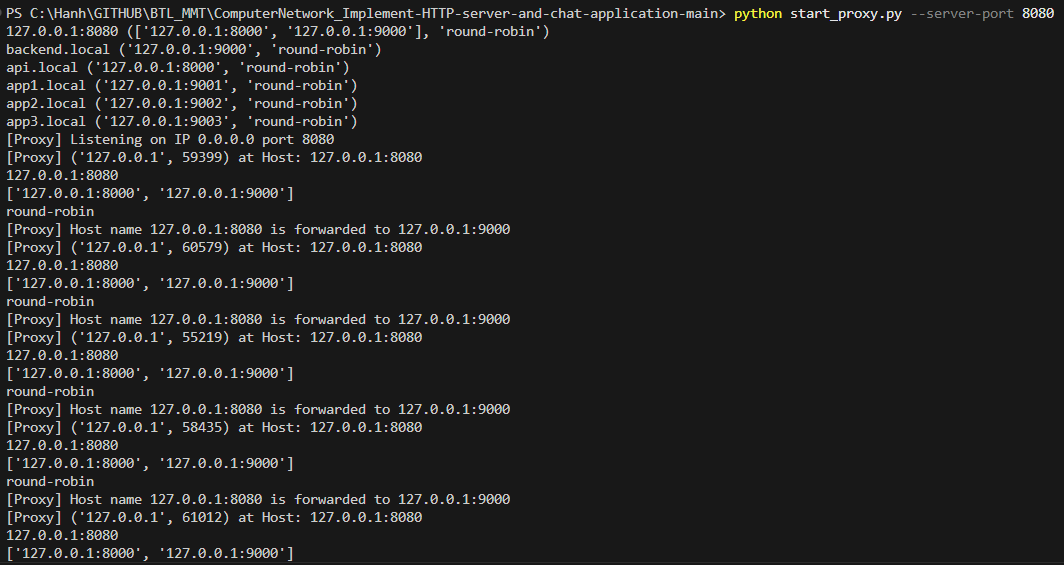
\includegraphics[width=\linewidth]{picture/proxyforward.png}
    \caption{Proxy}
    \label{fig:placeholder}
\end{figure}
\textbf{Gửi tin nhắn P2P qua Web UI:}
\begin{itemize}
    \item Người dùng ở \textbf{Client2 (UI)} nhấn gửi private message tới Client1; Web UI gọi \texttt{POST /send-peer} trên WebApp local (ví dụ \texttt{http://127.0.0.1:9002/send-peer}) với payload JSON \texttt{\{"from":"Client2","to":"Client1","message":"..."\}}.
    \item WebApp forwards request đến Proxy (8080) và Proxy forward tới Backend (9000). Backend lookup \texttt{Client1} trong \texttt{db/peer\_connections.json} để biết host:port.
    \item \textbf{Tùy trạng thái hệ thống:}
    \begin{itemize}
        \item Nếu backend và mạng nội bộ trả lời bình thường, backend/flow xác nhận và WebApp sẽ ghi log gửi/nhận; tùy cấu hình, backend có thể trả xác nhận mà không trực tiếp mở socket.
        \item Nếu backend không khả dụng hoặc WebApp cần gửi trực tiếp, WebApp sẽ thực hiện \textbf{TCP direct} tới host:port của Client1 (theo cache/file) bằng socket và gửi payload trực tiếp; Client1 sẽ nhận và hiển thị tin nhắn.
    \end{itemize}
    \item Mọi sự kiện gửi/nhận được ghi vào file log cục bộ: \texttt{db/Client1\_messages.json}, \texttt{db/Client2\_messages.json} (các entry có trường \texttt{direction} = \{send, recv, failed\}).
\end{itemize}
\begin{figure}[H]
    \centering
    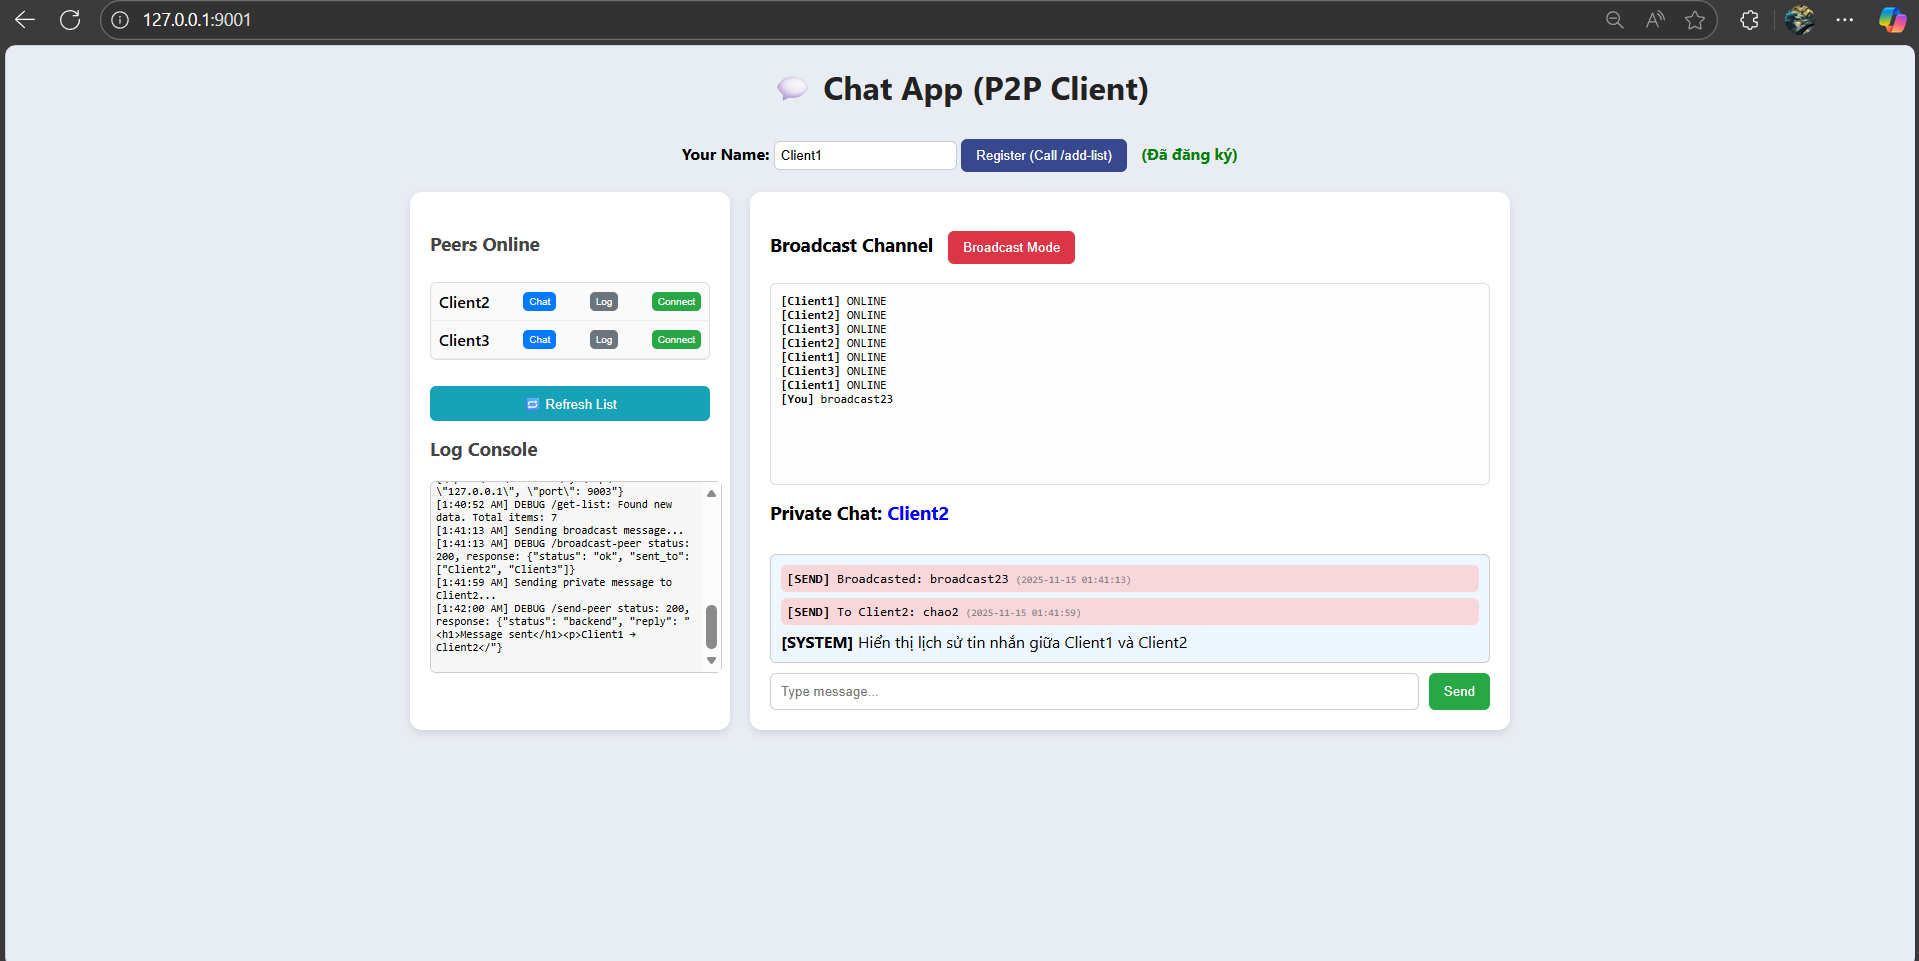
\includegraphics[width=\linewidth]{picture/logClient1.png}
    \caption{Log tin nhắn của Client1 khi backend hoạt động}
    \label{fig:placeholder}
\end{figure}
\begin{figure}[H]
    \centering
    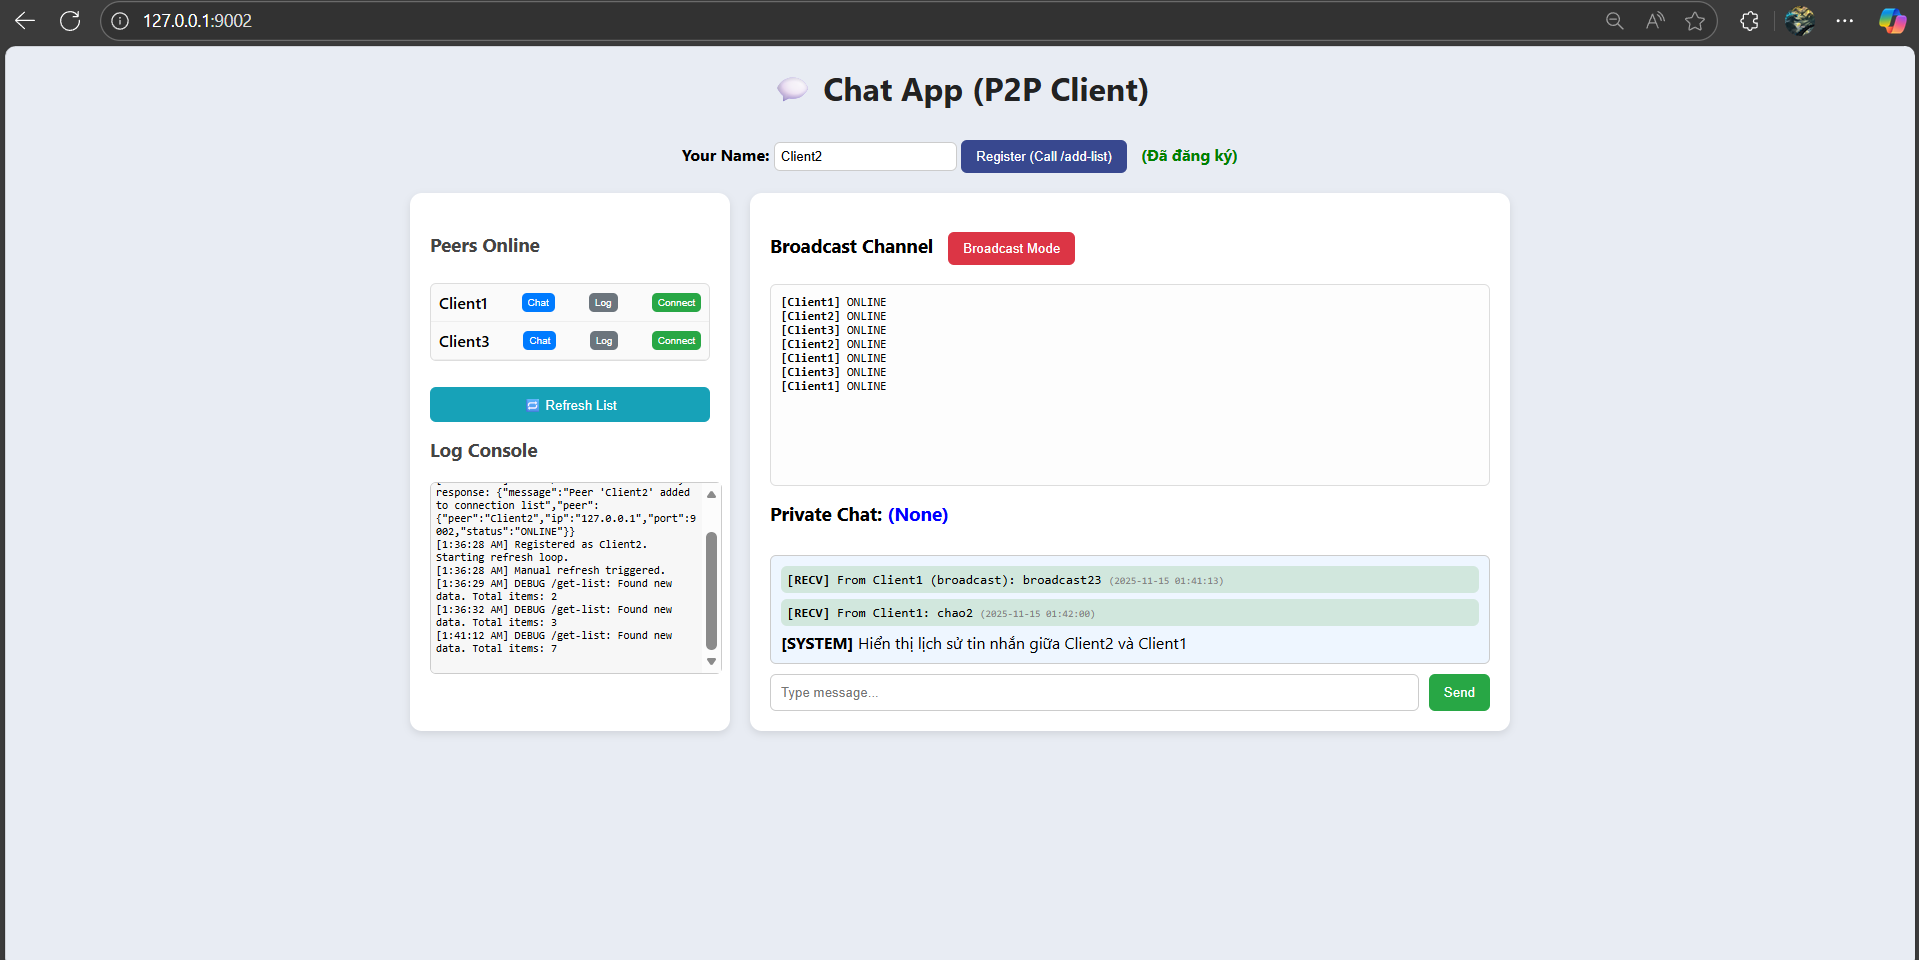
\includegraphics[width=\linewidth]{picture/logClient2.png}
    \caption{Log tin nhắn của Client2 khi backend hoạt động}
    \label{fig:placeholder}
\end{figure}
\begin{figure}[H]
    \centering
    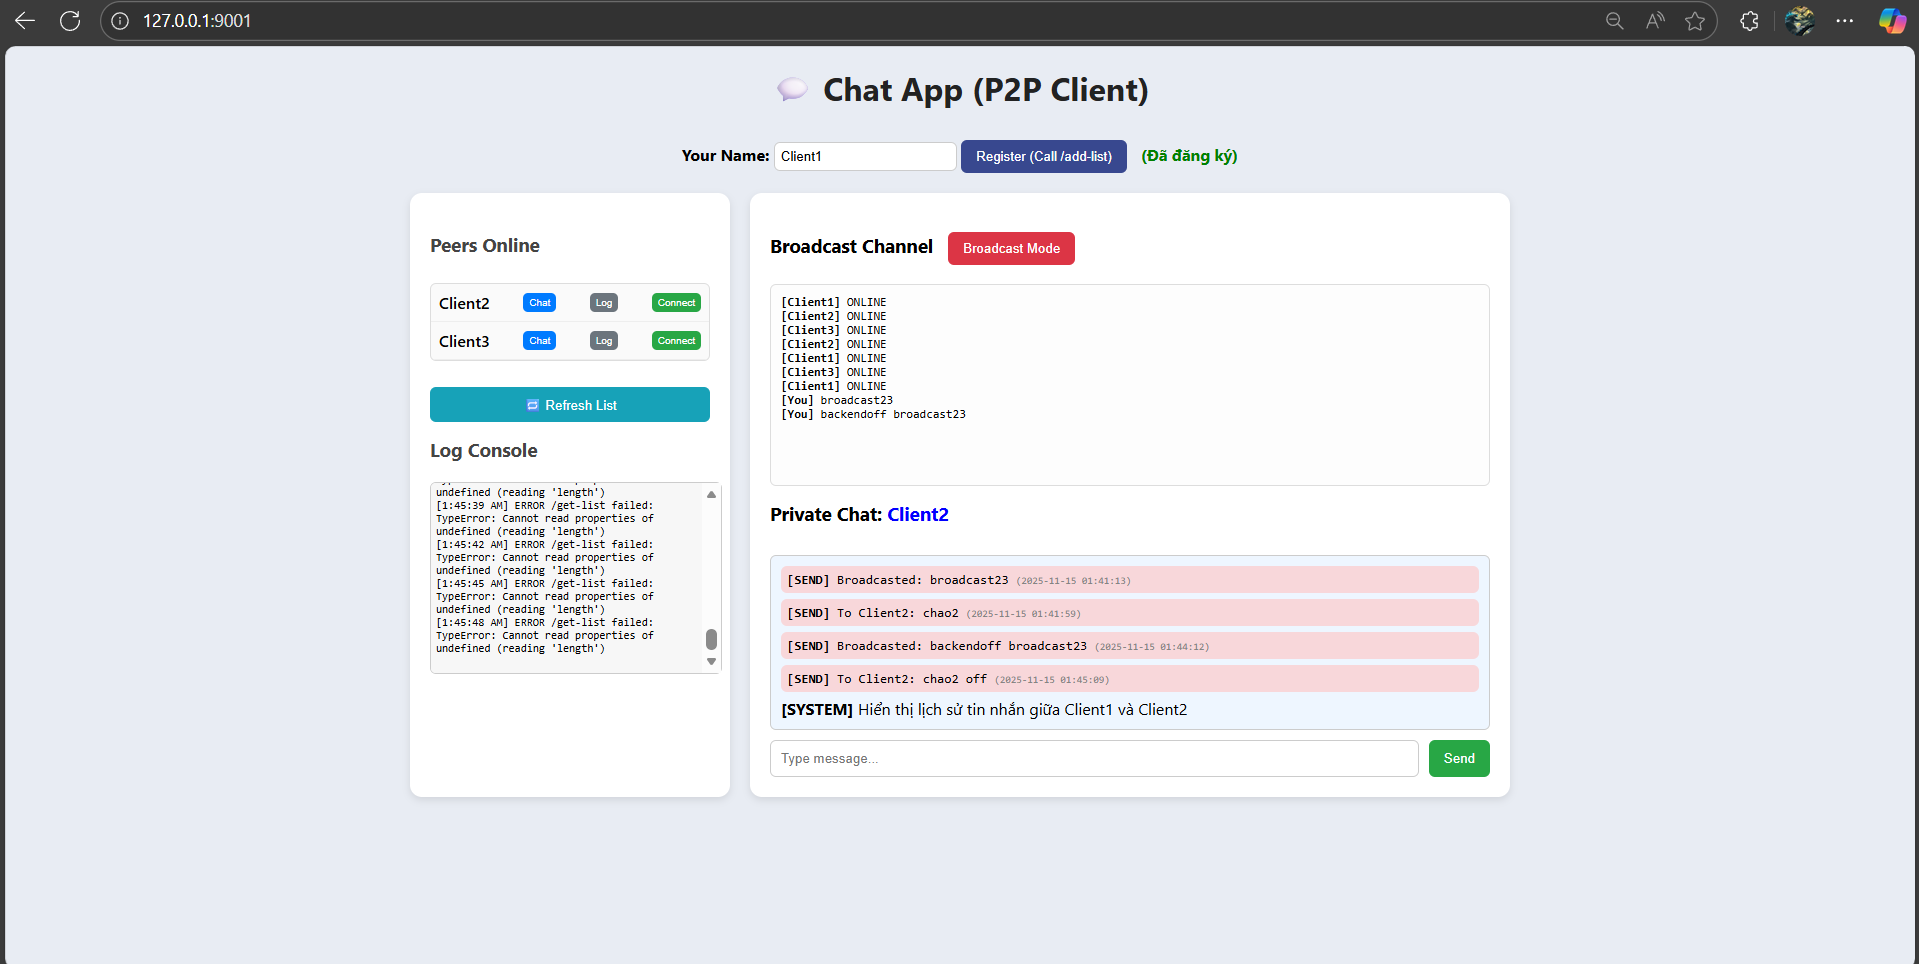
\includegraphics[width=\linewidth]{picture/logClient1off.png}
    \caption{Log tin nhắn của Client1 khi backend tắt}
    \label{fig:placeholder}
\end{figure}
\begin{figure}[H]
    \centering
    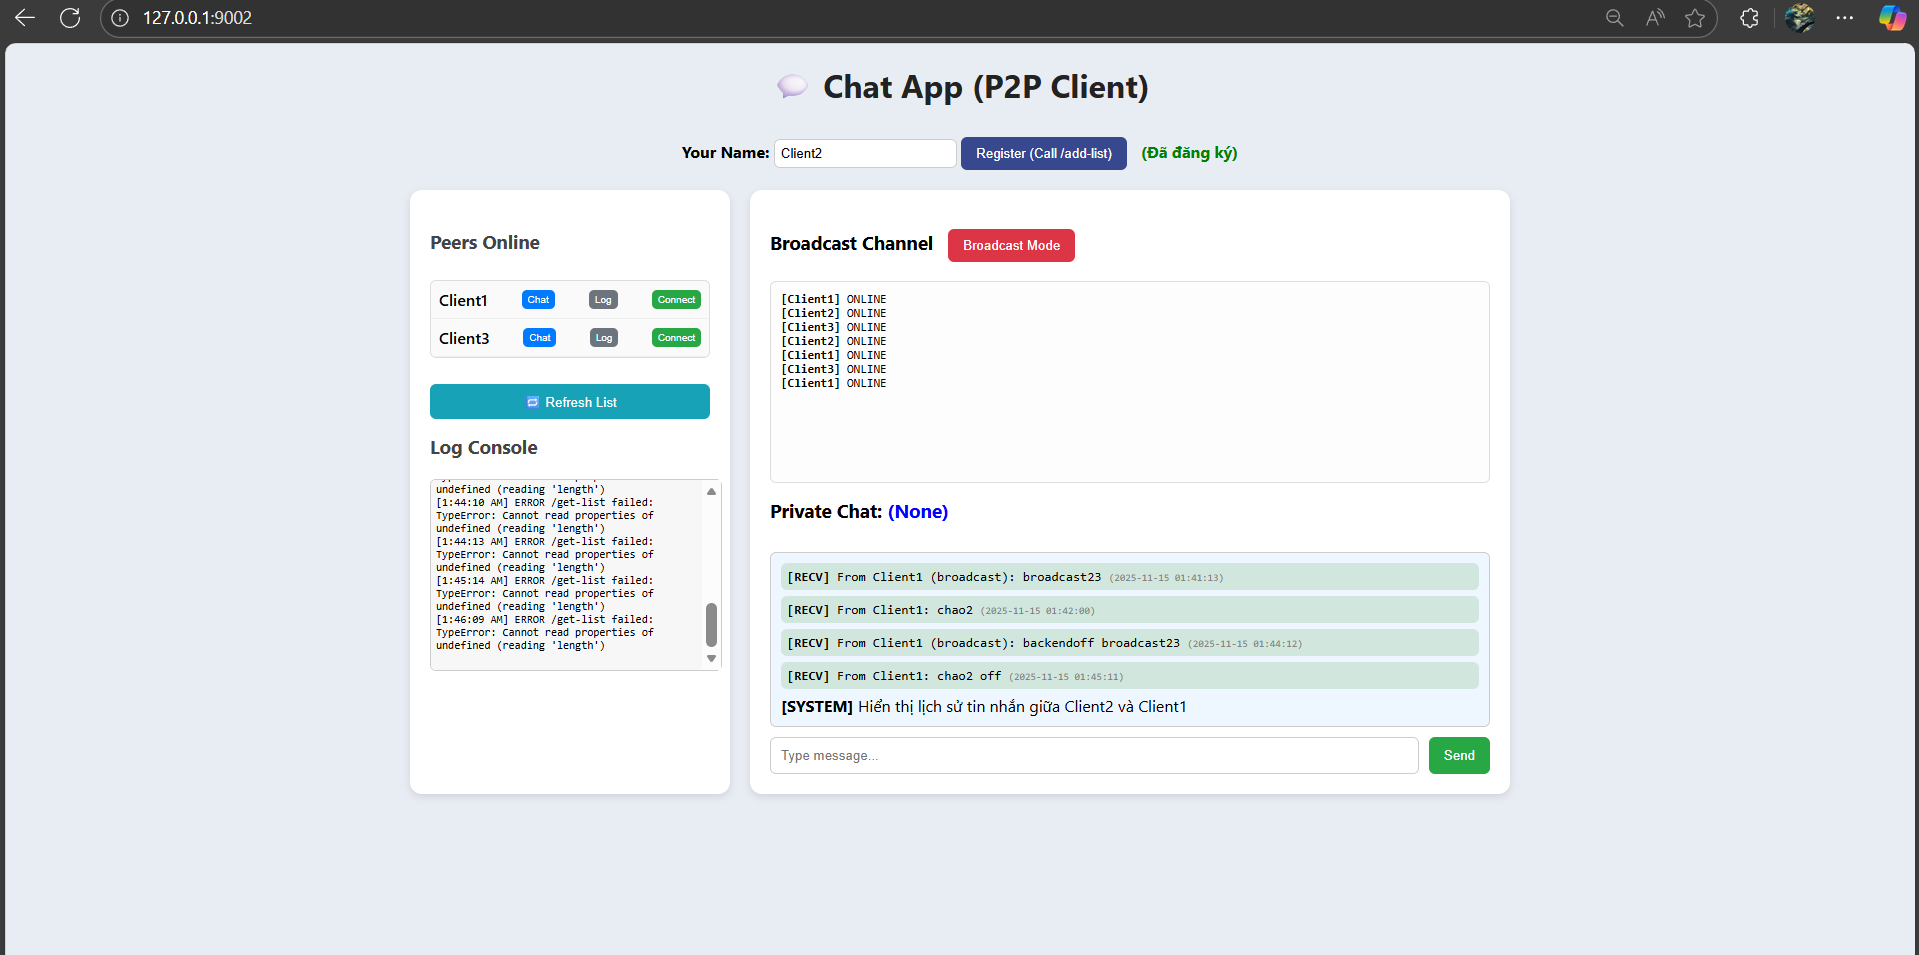
\includegraphics[width=\linewidth]{picture/logClient2off.png}
    \caption{Log tin nhắn của Client1 khi backend tắt}
    \label{fig:placeholder}
\end{figure}
\section{Hướng dẫn sử dụng}
\subsection{Chạy Backend}
Đầu tiên, khởi động tiến trình \textbf{Backend (Tracker)} để làm trung tâm quản lý danh sách các peer. 
Backend được triển khai trong file \texttt{start\_backend.py} và lắng nghe ở cổng \textbf{9000}. 

\textbf{Cách chạy:}
\begin{verbatim}
python start_backend.py --server-ip 127.0.0.1 --server-port 9000
\end{verbatim}

Sau khi khởi động thành công, màn hình sẽ hiển thị:
\begin{quote}
[Backend] Listening on port 9000
\end{quote}

Backend chịu trách nhiệm xử lý các request:
\begin{itemize}
    \item \texttt{/add-list}: đăng ký thông tin của peer.
    \item \texttt{/get-list}: trả về danh sách các peer đang hoạt động.
    \item \texttt{/connect-peer}, \texttt{/send-peer}: thiết lập hoặc gửi tin giữa các peer.
\end{itemize}
\subsection{Khởi động và cấu hình}
Mỗi peer được triển khai trong một tiến trình Python độc lập. Các peer này có thể chạy song song trên cùng máy tính. 
\begin{itemize}
    \item Chạy backend (tracker + các API):
    \begin{verbatim}
        py start_backend.py --server-ip 127.0.0.1 --server-port 9000
    \end{verbatim}
    \item Chạy proxy (reverse proxy lắng nghe client, forward theo proxy.conf):
    \begin{verbatim}
        py start_proxy.py --server-ip 127.0.0.1 --server-port 8080
    \end{verbatim}
    \item Chạy 3 peer — mỗi peer là một WebApp độc lập:
    \begin{verbatim}
        py start_sampleapp.py --server-ip 127.0.0.1 --server-port 9001
        py start_sampleapp.py --server-ip 127.0.0.1 --server-port 9002
        py start_sampleapp.py --server-ip 127.0.0.1 --server-port 9003
    \end{verbatim}
    \item Lưu ý routing: WebApp (start\_sampleapp) nội bộ cấu hình BACKEND\_URL = "http://127.0.0.1:8080" nên mọi API từ WebApp forward tới proxy(8080), proxy sẽ chuyển tiếp tới backend (9000) theo proxy.conf.
    \item Mỗi sampleapp khi call /add-list sẽ forward lên backend kèm host=app.ip và port=app.port (ví dụ 127.0.0.1:9001), nên backend lưu chính xác ip:port của peer trong db/peer\_connections.json.
    \item Nếu backend bị mất, WebApp dùng cache db/peers\_cache.json để giữ thông tin peer và fallback gửi trực tiếp TCP tới IP:port được lưu trong cache.
\end{itemize}
\subsection{Gửi và nhận tin nhắn}
Sau khi cả 3 peer đã đăng ký thành công vào tracker, ta có thể kiểm thử chức năng gửi và nhận tin nhắn thông qua endpoint \texttt{/send-peer}.

\textbf{Cách gửi tin bằng curl:}
\begin{verbatim}
curl -X POST http://127.0.0.1:9001/send-peer -H "Content-Type: application/json" -d "{\"from\":\"Client1\",\"to\":\"Client2\",\"message\":\"Hello Client2 from curl!\"}"
\end{verbatim}

\textbf{Kết quả:}
\begin{figure}[H]
    \centering
    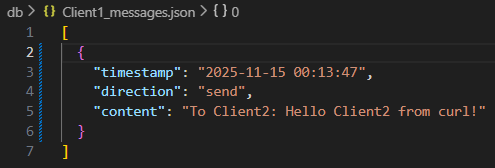
\includegraphics[width=\linewidth]{picture/client1mess.png}
    \caption{Client1\_messages.json}
    \label{fig:placeholder}
\end{figure}
\begin{figure}[H]
    \centering
    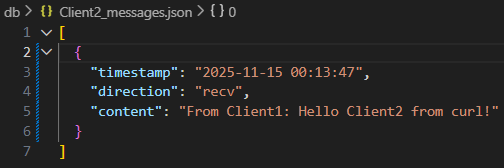
\includegraphics[width=\linewidth]{picture/client2mess.png}
    \caption{Client2\_messages.json}
    \label{fig:placeholder}
\end{figure}
/send-peer được gọi ở WebApp (hoặc client), WebApp gửi HTTP đến Proxy (127.0.0.1:8080), Proxy theo proxy.conf forward request tới Backend (127.0.0.1:9000), Backend đọc db/peer\_connections.json, xác định IP:port của peer đích và trả về xác nhận. Nếu backend không khả dụng, WebApp sẽ fallback gửi trực tiếp TCP tới peer theo cache.
\section{Kết luận và Hướng phát triển}
\subsection{Đánh giá kết quả}
Hệ thống đã \textbf{hoàn thành đầy đủ các mục tiêu} của Bài tập lớn Mạng Máy tính (CO3093/CO3094) với các điểm nổi bật sau:
\begin{itemize}
    \item \textbf{Hiện thực Mô hình Lai (Hybrid Paradigm):} Chứng minh được sự kết hợp giữa mô hình \textbf{Client-Server} (cho đăng ký, khám phá peer) và \textbf{Peer-to-Peer (P2P)} (cho truyền tin nhắn trực tiếp qua TCP Socket).
    \item \textbf{Bảo mật Cơ bản (Cookie Session):} Đã triển khai thành công cơ chế \textbf{xác thực} và \textbf{kiểm soát truy cập} bằng HTTP Cookies (Task 1).
    \item \textbf{Lập trình Mạng Nâng cao:} Đã vận dụng được lập trình socket TCP để xây dựng Proxy Server, các tiến trình Backend/Tracker, và kết nối P2P giữa các tiến trình.
\end{itemize}
\subsection{Hướng phát triển}
Để nâng cao tính thực tế và hiệu suất của ứng dụng, nhóm đề xuất các hướng phát triển trong tương lai:
\begin{itemize}
    \item \textbf{Chuyển đổi sang WebSockets/Server-Sent Events (SSE):} Thay vì sử dụng cơ chế \textbf{Polling (hỏi vòng)} cho Web Client (\texttt{/get-list}), nên chuyển sang sử dụng WebSockets hoặc SSE. Các công nghệ này cho phép Server \textbf{đẩy (push)} tin nhắn đến Client ngay lập tức, loại bỏ độ trễ và giảm tải cho Server.
    \item \textbf{Mã hóa Giao tiếp P2P:} Hiện tại, tin nhắn P2P được gửi dưới dạng văn bản thuần túy. Cần thêm cơ chế mã hóa (ví dụ: TLS/SSL) cho các kết nối socket giữa các peer để đảm bảo bảo mật dữ liệu.
    \item \textbf{Hỗ trợ NAT Traversal (Môi trường thực):} Tích hợp các kỹ thuật như \textbf{STUN/TURN/ICE} để các peer có thể thiết lập kết nối TCP trực tiếp thành công, ngay cả khi chúng nằm sau các thiết bị NAT/Firewall.
    \item \textbf{Tối ưu hóa Tracker:} Nâng cấp cấu trúc dữ liệu Tracker để hỗ trợ quản lý các \textbf{kênh (channels)} chat riêng, thay vì chỉ là một bảng tin toàn cục.
\end{itemize}
%\section{Tài liệu tham khảo}
\end{document}
